% VDE Template for EUSAR Papers
% Provided by Barbara Lang und Siegmar Lampe
% University of Bremen, January 2002
% English version by Jens Fischer
% German Aerospace Center (DLR), December 2005
% Additional modifications by Matthias Wei{\ss}
% FGAN, January 2009

%-----------------------------------------------------------------------------
% Type of publication
\documentclass[a4paper,10pt]{article}
%-----------------------------------------------------------------------------
% Other packets: Most packets may be downloaded from www.dante.de and
% "tcilatex.tex" can be found at (December 2005):
% http://www.mackichan.com/techtalk/v30/UsingFloat.htm
% Not all packets are necessarily needed:
\usepackage[T1]{fontenc}
\usepackage[latin1]{inputenc}
%\usepackage{ngerman} % in german language if required
\usepackage[nooneline,bf]{caption} % Figure descriptions from left margin
\usepackage{times}
\usepackage{multicol}
\usepackage{amsmath}
\usepackage{amssymb}
\usepackage{graphicx}
\usepackage{epsfig}
\usepackage{listings}
\usepackage{color}
\usepackage{nameref}
\usepackage{url}
\usepackage{inconsolata}
\usepackage{dirtree}
\usepackage[firstpage]{draftwatermark}
%\usepackage{draftwatermark}
\SetWatermarkLightness{0.84}
%\usepackage{paralist}

% Macros for Scientific Word 3.0 documents saved with the LaTeX filter.
%Copyright (C) 1994-97 TCI Software Research, Inc.
\typeout{TCILATEX Macros for Scientific Word 3.0 <05 August 1998>.}
\typeout{NOTICE:  This macro file is NOT proprietary and may be 
freely copied and distributed.}
%
\makeatletter
%
%%%%%%%%%%%%%%%%%%%%%%
% macros for time
\newcount\@hour\newcount\@minute\chardef\@x10\chardef\@xv60
\def\tcitime{
\def\@time{%
  \@minute\time\@hour\@minute\divide\@hour\@xv
  \ifnum\@hour<\@x 0\fi\the\@hour:%
  \multiply\@hour\@xv\advance\@minute-\@hour
  \ifnum\@minute<\@x 0\fi\the\@minute
  }}%

%%%%%%%%%%%%%%%%%%%%%%
% macro for hyperref
\@ifundefined{hyperref}{\def\hyperref#1#2#3#4{#2\ref{#4}#3}}{}

% macro for external program call
\@ifundefined{qExtProgCall}{\def\qExtProgCall#1#2#3#4#5#6{\relax}}{}
%%%%%%%%%%%%%%%%%%%%%%
%
% macros for graphics
%
\def\FILENAME#1{#1}%
%
\def\QCTOpt[#1]#2{%
  \def\QCTOptB{#1}
  \def\QCTOptA{#2}
}
\def\QCTNOpt#1{%
  \def\QCTOptA{#1}
  \let\QCTOptB\empty
}
\def\Qct{%
  \@ifnextchar[{%
    \QCTOpt}{\QCTNOpt}
}
\def\QCBOpt[#1]#2{%
  \def\QCBOptB{#1}
  \def\QCBOptA{#2}
}
\def\QCBNOpt#1{%
  \def\QCBOptA{#1}
  \let\QCBOptB\empty
}
\def\Qcb{%
  \@ifnextchar[{%
    \QCBOpt}{\QCBNOpt}
}
\def\PrepCapArgs{%
  \ifx\QCBOptA\empty
    \ifx\QCTOptA\empty
      {}%
    \else
      \ifx\QCTOptB\empty
        {\QCTOptA}%
      \else
        [\QCTOptB]{\QCTOptA}%
      \fi
    \fi
  \else
    \ifx\QCBOptA\empty
      {}%
    \else
      \ifx\QCBOptB\empty
        {\QCBOptA}%
      \else
        [\QCBOptB]{\QCBOptA}%
      \fi
    \fi
  \fi
}
\newcount\GRAPHICSTYPE
%\GRAPHICSTYPE 0 is for TurboTeX
%\GRAPHICSTYPE 1 is for DVIWindo (PostScript)
%%%(removed)%\GRAPHICSTYPE 2 is for psfig (PostScript)
\GRAPHICSTYPE=\z@
\def\GRAPHICSPS#1{%
 \ifcase\GRAPHICSTYPE%\GRAPHICSTYPE=0
   \special{ps: #1}%
 \or%\GRAPHICSTYPE=1
   \special{language "PS", include "#1"}%
%%%\or%\GRAPHICSTYPE=2
%%%  #1%
 \fi
}%
%
\def\GRAPHICSHP#1{\special{include #1}}%
%
% \graffile{ body }                                  %#1
%          { contentswidth (scalar)  }               %#2
%          { contentsheight (scalar) }               %#3
%          { vertical shift when in-line (scalar) }  %#4
\def\graffile#1#2#3#4{%
%%% \ifnum\GRAPHICSTYPE=\tw@
%%%  %Following if using psfig
%%%  \@ifundefined{psfig}{\input psfig.tex}{}%
%%%  \psfig{file=#1, height=#3, width=#2}%
%%% \else
  %Following for all others
  % JCS - added BOXTHEFRAME, see below
    \bgroup
    \leavevmode
    \@ifundefined{bbl@deactivate}{\def~{\string~}}{\activesoff}
    \raise -#4 \BOXTHEFRAME{%
        \hbox to #2{\raise #3\hbox to #2{\null #1\hfil}}}%
    \egroup
}%
%
% A box for drafts
\def\draftbox#1#2#3#4{%
 \leavevmode\raise -#4 \hbox{%
  \frame{\rlap{\protect\tiny #1}\hbox to #2%
   {\vrule height#3 width\z@ depth\z@\hfil}%
  }%
 }%
}%
%
\newcount\draft
\draft=\z@
\let\nographics=\draft
\newif\ifwasdraft
\wasdraftfalse

%  \GRAPHIC{ body }                                  %#1
%          { draft name }                            %#2
%          { contentswidth (scalar)  }               %#3
%          { contentsheight (scalar) }               %#4
%          { vertical shift when in-line (scalar) }  %#5
\def\GRAPHIC#1#2#3#4#5{%
 \ifnum\draft=\@ne\draftbox{#2}{#3}{#4}{#5}%
  \else\graffile{#1}{#3}{#4}{#5}%
  \fi
 }%
%
\def\addtoLaTeXparams#1{%
    \edef\LaTeXparams{\LaTeXparams #1}}%
%
% JCS -  added a switch BoxFrame that can 
% be set by including X in the frame params.
% If set a box is drawn around the frame.

\newif\ifBoxFrame \BoxFramefalse
\newif\ifOverFrame \OverFramefalse
\newif\ifUnderFrame \UnderFramefalse

\def\BOXTHEFRAME#1{%
   \hbox{%
      \ifBoxFrame
         \frame{#1}%
      \else
         {#1}%
      \fi
   }%
}


\def\doFRAMEparams#1{\BoxFramefalse\OverFramefalse\UnderFramefalse\readFRAMEparams#1\end}%
\def\readFRAMEparams#1{%
 \ifx#1\end%
  \let\next=\relax
  \else
  \ifx#1i\dispkind=\z@\fi
  \ifx#1d\dispkind=\@ne\fi
  \ifx#1f\dispkind=\tw@\fi
  \ifx#1t\addtoLaTeXparams{t}\fi
  \ifx#1b\addtoLaTeXparams{b}\fi
  \ifx#1p\addtoLaTeXparams{p}\fi
  \ifx#1h\addtoLaTeXparams{h}\fi
  \ifx#1X\BoxFrametrue\fi
  \ifx#1O\OverFrametrue\fi
  \ifx#1U\UnderFrametrue\fi
  \ifx#1w
    \ifnum\draft=1\wasdrafttrue\else\wasdraftfalse\fi
    \draft=\@ne
  \fi
  \let\next=\readFRAMEparams
  \fi
 \next
 }%
%
%Macro for In-line graphics object
%   \IFRAME{ contentswidth (scalar)  }               %#1
%          { contentsheight (scalar) }               %#2
%          { vertical shift when in-line (scalar) }  %#3
%          { draft name }                            %#4
%          { body }                                  %#5
%          { caption}                                %#6


\def\IFRAME#1#2#3#4#5#6{%
      \bgroup
      \let\QCTOptA\empty
      \let\QCTOptB\empty
      \let\QCBOptA\empty
      \let\QCBOptB\empty
      #6%
      \parindent=0pt%
      \leftskip=0pt
      \rightskip=0pt
      \setbox0 = \hbox{\QCBOptA}%
      \@tempdima = #1\relax
      \ifOverFrame
          % Do this later
          \typeout{This is not implemented yet}%
          \show\HELP
      \else
         \ifdim\wd0>\@tempdima
            \advance\@tempdima by \@tempdima
            \ifdim\wd0 >\@tempdima
               \textwidth=\@tempdima
               \setbox1 =\vbox{%
                  \noindent\hbox to \@tempdima{\hfill\GRAPHIC{#5}{#4}{#1}{#2}{#3}\hfill}\\%
                  \noindent\hbox to \@tempdima{\parbox[b]{\@tempdima}{\QCBOptA}}%
               }%
               \wd1=\@tempdima
            \else
               \textwidth=\wd0
               \setbox1 =\vbox{%
                 \noindent\hbox to \wd0{\hfill\GRAPHIC{#5}{#4}{#1}{#2}{#3}\hfill}\\%
                 \noindent\hbox{\QCBOptA}%
               }%
               \wd1=\wd0
            \fi
         \else
            %\show\BBB
            \ifdim\wd0>0pt
              \hsize=\@tempdima
              \setbox1 =\vbox{%
                \unskip\GRAPHIC{#5}{#4}{#1}{#2}{0pt}%
                \break
                \unskip\hbox to \@tempdima{\hfill \QCBOptA\hfill}%
              }%
              \wd1=\@tempdima
           \else
              \hsize=\@tempdima
              \setbox1 =\vbox{%
                \unskip\GRAPHIC{#5}{#4}{#1}{#2}{0pt}%
              }%
              \wd1=\@tempdima
           \fi
         \fi
         \@tempdimb=\ht1
         \advance\@tempdimb by \dp1
         \advance\@tempdimb by -#2%
         \advance\@tempdimb by #3%
         \leavevmode
         \raise -\@tempdimb \hbox{\box1}%
      \fi
      \egroup%
}%
%
%Macro for Display graphics object
%   \DFRAME{ contentswidth (scalar)  }               %#1
%          { contentsheight (scalar) }               %#2
%          { draft label }                           %#3
%          { name }                                  %#4
%          { caption}                                %#5
\def\DFRAME#1#2#3#4#5{%
 \begin{center}
     \let\QCTOptA\empty
     \let\QCTOptB\empty
     \let\QCBOptA\empty
     \let\QCBOptB\empty
     \ifOverFrame 
        #5\QCTOptA\par
     \fi
     \GRAPHIC{#4}{#3}{#1}{#2}{\z@}
     \ifUnderFrame 
        \nobreak\par\nobreak#5\QCBOptA
     \fi
 \end{center}%
 }%
%
%Macro for Floating graphic object
%   \FFRAME{ framedata f|i tbph x F|T }              %#1
%          { contentswidth (scalar)  }               %#2
%          { contentsheight (scalar) }               %#3
%          { caption }                               %#4
%          { label }                                 %#5
%          { draft name }                            %#6
%          { body }                                  %#7
\def\FFRAME#1#2#3#4#5#6#7{%
 %If float.sty loaded and float option is 'h', change to 'H'  (gp) 1998/09/05
  \@ifundefined{floatstyle}
    {%floatstyle undefined (and float.sty not present), no change
     \begin{figure}[#1]%
    }
    {%floatstyle DEFINED
	 \ifx#1h%Only the h parameter, change to H
      \begin{figure}[H]%
	 \else
      \begin{figure}[#1]%
	 \fi
	}
  \let\QCTOptA\empty
  \let\QCTOptB\empty
  \let\QCBOptA\empty
  \let\QCBOptB\empty
  \ifOverFrame
    #4
    \ifx\QCTOptA\empty
    \else
      \ifx\QCTOptB\empty
        \caption{\QCTOptA}%
      \else
        \caption[\QCTOptB]{\QCTOptA}%
      \fi
    \fi
    \ifUnderFrame\else
      \label{#5}%
    \fi
  \else
    \UnderFrametrue%
  \fi
  \begin{center}\GRAPHIC{#7}{#6}{#2}{#3}{\z@}\end{center}%
  \ifUnderFrame
    #4
    \ifx\QCBOptA\empty
      \caption{}%
    \else
      \ifx\QCBOptB\empty
        \caption{\QCBOptA}%
      \else
        \caption[\QCBOptB]{\QCBOptA}%
      \fi
    \fi
    \label{#5}%
  \fi
  \end{figure}%
 }%
%
%
%    \FRAME{ framedata f|i tbph x F|T }              %#1
%          { contentswidth (scalar)  }               %#2
%          { contentsheight (scalar) }               %#3
%          { vertical shift when in-line (scalar) }  %#4
%          { caption }                               %#5
%          { label }                                 %#6
%          { name }                                  %#7
%          { body }                                  %#8
%
%    framedata is a string which can contain the following
%    characters: idftbphxFT
%    Their meaning is as follows:
%             i, d or f : in-line, display, or floating
%             t,b,p,h   : LaTeX floating placement options
%             x         : fit contents box to contents
%             F or T    : Figure or Table. 
%                         Later this can expand
%                         to a more general float class.
%
%
\newcount\dispkind%

\def\makeactives{
  \catcode`\"=\active
  \catcode`\;=\active
  \catcode`\:=\active
  \catcode`\'=\active
  \catcode`\~=\active
}
\bgroup
   \makeactives
   \gdef\activesoff{%
      \def"{\string"}
      \def;{\string;}
      \def:{\string:}
      \def'{\string'}
      \def~{\string~}
      %\bbl@deactivate{"}%
      %\bbl@deactivate{;}%
      %\bbl@deactivate{:}%
      %\bbl@deactivate{'}%
    }
\egroup

\def\FRAME#1#2#3#4#5#6#7#8{%
 \bgroup
 \ifnum\draft=\@ne
   \wasdrafttrue
 \else
   \wasdraftfalse%
 \fi
 \def\LaTeXparams{}%
 \dispkind=\z@
 \def\LaTeXparams{}%
 \doFRAMEparams{#1}%
 \ifnum\dispkind=\z@\IFRAME{#2}{#3}{#4}{#7}{#8}{#5}\else
  \ifnum\dispkind=\@ne\DFRAME{#2}{#3}{#7}{#8}{#5}\else
   \ifnum\dispkind=\tw@
    \edef\@tempa{\noexpand\FFRAME{\LaTeXparams}}%
    \@tempa{#2}{#3}{#5}{#6}{#7}{#8}%
    \fi
   \fi
  \fi
  \ifwasdraft\draft=1\else\draft=0\fi{}%
  \egroup
 }%
%
% This macro added to let SW gobble a parameter that
% should not be passed on and expanded. 

\def\TEXUX#1{"texux"}

%
% Macros for text attributes:
%
\def\BF#1{{\bf {#1}}}%
\def\NEG#1{\leavevmode\hbox{\rlap{\thinspace/}{$#1$}}}%
%
%%%%%%%%%%%%%%%%%%%%%%%%%%%%%%%%%%%%%%%%%%%%%%%%%%%%%%%%%%%%%%%%%%%%%%%%
%
%
% macros for user - defined functions
\def\limfunc#1{\mathop{\rm #1}}%
\def\func#1{\mathop{\rm #1}\nolimits}%
% macro for unit names
\def\unit#1{\mathop{\rm #1}\nolimits}%

%
% miscellaneous 
\long\def\QQQ#1#2{%
     \long\expandafter\def\csname#1\endcsname{#2}}%
\@ifundefined{QTP}{\def\QTP#1{}}{}
\@ifundefined{QEXCLUDE}{\def\QEXCLUDE#1{}}{}
\@ifundefined{Qlb}{\def\Qlb#1{#1}}{}
\@ifundefined{Qlt}{\def\Qlt#1{#1}}{}
\def\QWE{}%
\long\def\QQA#1#2{}%
\def\QTR#1#2{{\csname#1\endcsname #2}}%(gp) Is this the best?
\long\def\TeXButton#1#2{#2}%
\long\def\QSubDoc#1#2{#2}%
\def\EXPAND#1[#2]#3{}%
\def\NOEXPAND#1[#2]#3{}%
\def\PROTECTED{}%
\def\LaTeXparent#1{}%
\def\ChildStyles#1{}%
\def\ChildDefaults#1{}%
\def\QTagDef#1#2#3{}%

% Constructs added with Scientific Notebook
\@ifundefined{correctchoice}{\def\correctchoice{\relax}}{}
\@ifundefined{HTML}{\def\HTML#1{\relax}}{}
\@ifundefined{TCIIcon}{\def\TCIIcon#1#2#3#4{\relax}}{}
\if@compatibility
  \typeout{Not defining UNICODE or CustomNote commands for LaTeX 2.09.}
\else
  \providecommand{\UNICODE}[2][]{}
  \providecommand{\CustomNote}[3][]{\marginpar{#3}}
\fi

%
% Macros for style editor docs
\@ifundefined{StyleEditBeginDoc}{\def\StyleEditBeginDoc{\relax}}{}
%
% Macros for footnotes
\def\QQfnmark#1{\footnotemark}
\def\QQfntext#1#2{\addtocounter{footnote}{#1}\footnotetext{#2}}
%
% Macros for indexing.
%
\@ifundefined{TCIMAKEINDEX}{}{\makeindex}%
%
% Attempts to avoid problems with other styles
\@ifundefined{abstract}{%
 \def\abstract{%
  \if@twocolumn
   \section*{Abstract (Not appropriate in this style!)}%
   \else \small 
   \begin{center}{\bf Abstract\vspace{-.5em}\vspace{\z@}}\end{center}%
   \quotation 
   \fi
  }%
 }{%
 }%
\@ifundefined{endabstract}{\def\endabstract
  {\if@twocolumn\else\endquotation\fi}}{}%
\@ifundefined{maketitle}{\def\maketitle#1{}}{}%
\@ifundefined{affiliation}{\def\affiliation#1{}}{}%
\@ifundefined{proof}{\def\proof{\noindent{\bfseries Proof. }}}{}%
\@ifundefined{endproof}{\def\endproof{\mbox{\ \rule{.1in}{.1in}}}}{}%
\@ifundefined{newfield}{\def\newfield#1#2{}}{}%
\@ifundefined{chapter}{\def\chapter#1{\par(Chapter head:)#1\par }%
 \newcount\c@chapter}{}%
\@ifundefined{part}{\def\part#1{\par(Part head:)#1\par }}{}%
\@ifundefined{section}{\def\section#1{\par(Section head:)#1\par }}{}%
\@ifundefined{subsection}{\def\subsection#1%
 {\par(Subsection head:)#1\par }}{}%
\@ifundefined{subsubsection}{\def\subsubsection#1%
 {\par(Subsubsection head:)#1\par }}{}%
\@ifundefined{paragraph}{\def\paragraph#1%
 {\par(Subsubsubsection head:)#1\par }}{}%
\@ifundefined{subparagraph}{\def\subparagraph#1%
 {\par(Subsubsubsubsection head:)#1\par }}{}%
%%%%%%%%%%%%%%%%%%%%%%%%%%%%%%%%%%%%%%%%%%%%%%%%%%%%%%%%%%%%%%%%%%%%%%%%
% These symbols are not recognized by LaTeX
\@ifundefined{therefore}{\def\therefore{}}{}%
\@ifundefined{backepsilon}{\def\backepsilon{}}{}%
\@ifundefined{yen}{\def\yen{\hbox{\rm\rlap=Y}}}{}%
\@ifundefined{registered}{%
   \def\registered{\relax\ifmmode{}\r@gistered
                    \else$\m@th\r@gistered$\fi}%
 \def\r@gistered{^{\ooalign
  {\hfil\raise.07ex\hbox{$\scriptstyle\rm\text{R}$}\hfil\crcr
  \mathhexbox20D}}}}{}%
\@ifundefined{Eth}{\def\Eth{}}{}%
\@ifundefined{eth}{\def\eth{}}{}%
\@ifundefined{Thorn}{\def\Thorn{}}{}%
\@ifundefined{thorn}{\def\thorn{}}{}%
% A macro to allow any symbol that requires math to appear in text
\def\TEXTsymbol#1{\mbox{$#1$}}%
\@ifundefined{degree}{\def\degree{{}^{\circ}}}{}%
%
% macros for T3TeX files
\newdimen\theight
\def\Column{%
 \vadjust{\setbox\z@=\hbox{\scriptsize\quad\quad tcol}%
  \theight=\ht\z@\advance\theight by \dp\z@\advance\theight by \lineskip
  \kern -\theight \vbox to \theight{%
   \rightline{\rlap{\box\z@}}%
   \vss
   }%
  }%
 }%
%
\def\qed{%
 \ifhmode\unskip\nobreak\fi\ifmmode\ifinner\else\hskip5\p@\fi\fi
 \hbox{\hskip5\p@\vrule width4\p@ height6\p@ depth1.5\p@\hskip\p@}%
 }%
%
\def\cents{\hbox{\rm\rlap/c}}%
\def\miss{\hbox{\vrule height2\p@ width 2\p@ depth\z@}}%
%
\def\vvert{\Vert}%           %always translated to \left| or \right|
%
\def\tcol#1{{\baselineskip=6\p@ \vcenter{#1}} \Column}  %
%
\def\dB{\hbox{{}}}%                 %dummy entry in column 
\def\mB#1{\hbox{$#1$}}%             %column entry
\def\nB#1{\hbox{#1}}%               %column entry (not math)
%
\@ifundefined{note}{\def\note{$^{\dag}}}{}%
%

\def\newfmtname{LaTeX2e}
% No longer load latexsym.  This is now handled by SWP, which uses amsfonts if necessary

\ifx\fmtname\newfmtname
  \DeclareOldFontCommand{\rm}{\normalfont\rmfamily}{\mathrm}
  \DeclareOldFontCommand{\sf}{\normalfont\sffamily}{\mathsf}
  \DeclareOldFontCommand{\tt}{\normalfont\ttfamily}{\mathtt}
  \DeclareOldFontCommand{\bf}{\normalfont\bfseries}{\mathbf}
  \DeclareOldFontCommand{\it}{\normalfont\itshape}{\mathit}
  \DeclareOldFontCommand{\sl}{\normalfont\slshape}{\@nomath\sl}
  \DeclareOldFontCommand{\sc}{\normalfont\scshape}{\@nomath\sc}
\fi

%
% Greek bold macros
% Redefine all of the math symbols 
% which might be bolded	 - there are 
% probably others to add to this list

\def\alpha{{\Greekmath 010B}}%
\def\beta{{\Greekmath 010C}}%
\def\gamma{{\Greekmath 010D}}%
\def\delta{{\Greekmath 010E}}%
\def\epsilon{{\Greekmath 010F}}%
\def\zeta{{\Greekmath 0110}}%
\def\eta{{\Greekmath 0111}}%
\def\theta{{\Greekmath 0112}}%
\def\iota{{\Greekmath 0113}}%
\def\kappa{{\Greekmath 0114}}%
\def\lambda{{\Greekmath 0115}}%
\def\mu{{\Greekmath 0116}}%
\def\nu{{\Greekmath 0117}}%
\def\xi{{\Greekmath 0118}}%
\def\pi{{\Greekmath 0119}}%
\def\rho{{\Greekmath 011A}}%
\def\sigma{{\Greekmath 011B}}%
\def\tau{{\Greekmath 011C}}%
\def\upsilon{{\Greekmath 011D}}%
\def\phi{{\Greekmath 011E}}%
\def\chi{{\Greekmath 011F}}%
\def\psi{{\Greekmath 0120}}%
\def\omega{{\Greekmath 0121}}%
\def\varepsilon{{\Greekmath 0122}}%
\def\vartheta{{\Greekmath 0123}}%
\def\varpi{{\Greekmath 0124}}%
\def\varrho{{\Greekmath 0125}}%
\def\varsigma{{\Greekmath 0126}}%
\def\varphi{{\Greekmath 0127}}%

\def\nabla{{\Greekmath 0272}}
\def\FindBoldGroup{%
   {\setbox0=\hbox{$\mathbf{x\global\edef\theboldgroup{\the\mathgroup}}$}}%
}

\def\Greekmath#1#2#3#4{%
    \if@compatibility
        \ifnum\mathgroup=\symbold
           \mathchoice{\mbox{\boldmath$\displaystyle\mathchar"#1#2#3#4$}}%
                      {\mbox{\boldmath$\textstyle\mathchar"#1#2#3#4$}}%
                      {\mbox{\boldmath$\scriptstyle\mathchar"#1#2#3#4$}}%
                      {\mbox{\boldmath$\scriptscriptstyle\mathchar"#1#2#3#4$}}%
        \else
           \mathchar"#1#2#3#4% 
        \fi 
    \else 
        \FindBoldGroup
        \ifnum\mathgroup=\theboldgroup % For 2e
           \mathchoice{\mbox{\boldmath$\displaystyle\mathchar"#1#2#3#4$}}%
                      {\mbox{\boldmath$\textstyle\mathchar"#1#2#3#4$}}%
                      {\mbox{\boldmath$\scriptstyle\mathchar"#1#2#3#4$}}%
                      {\mbox{\boldmath$\scriptscriptstyle\mathchar"#1#2#3#4$}}%
        \else
           \mathchar"#1#2#3#4% 
        \fi     	    
	  \fi}

\newif\ifGreekBold  \GreekBoldfalse
\let\SAVEPBF=\pbf
\def\pbf{\GreekBoldtrue\SAVEPBF}%
%

\@ifundefined{theorem}{\newtheorem{theorem}{Theorem}}{}
\@ifundefined{lemma}{\newtheorem{lemma}[theorem]{Lemma}}{}
\@ifundefined{corollary}{\newtheorem{corollary}[theorem]{Corollary}}{}
\@ifundefined{conjecture}{\newtheorem{conjecture}[theorem]{Conjecture}}{}
\@ifundefined{proposition}{\newtheorem{proposition}[theorem]{Proposition}}{}
\@ifundefined{axiom}{\newtheorem{axiom}{Axiom}}{}
\@ifundefined{remark}{\newtheorem{remark}{Remark}}{}
\@ifundefined{example}{\newtheorem{example}{Example}}{}
\@ifundefined{exercise}{\newtheorem{exercise}{Exercise}}{}
\@ifundefined{definition}{\newtheorem{definition}{Definition}}{}


\@ifundefined{mathletters}{%
  %\def\theequation{\arabic{equation}}
  \newcounter{equationnumber}  
  \def\mathletters{%
     \addtocounter{equation}{1}
     \edef\@currentlabel{\theequation}%
     \setcounter{equationnumber}{\c@equation}
     \setcounter{equation}{0}%
     \edef\theequation{\@currentlabel\noexpand\alph{equation}}%
  }
  \def\endmathletters{%
     \setcounter{equation}{\value{equationnumber}}%
  }
}{}

%Logos
\@ifundefined{BibTeX}{%
    \def\BibTeX{{\rm B\kern-.05em{\sc i\kern-.025em b}\kern-.08em
                 T\kern-.1667em\lower.7ex\hbox{E}\kern-.125emX}}}{}%
\@ifundefined{AmS}%
    {\def\AmS{{\protect\usefont{OMS}{cmsy}{m}{n}%
                A\kern-.1667em\lower.5ex\hbox{M}\kern-.125emS}}}{}%
\@ifundefined{AmSTeX}{\def\AmSTeX{\protect\AmS-\protect\TeX\@}}{}%
%

% This macro is a fix to eqnarray
\def\@@eqncr{\let\@tempa\relax
    \ifcase\@eqcnt \def\@tempa{& & &}\or \def\@tempa{& &}%
      \else \def\@tempa{&}\fi
     \@tempa
     \if@eqnsw
        \iftag@
           \@taggnum
        \else
           \@eqnnum\stepcounter{equation}%
        \fi
     \fi
     \global\tag@false
     \global\@eqnswtrue
     \global\@eqcnt\z@\cr}


\def\TCItag{\@ifnextchar*{\@TCItagstar}{\@TCItag}}
\def\@TCItag#1{%
    \global\tag@true
    \global\def\@taggnum{(#1)}}
\def\@TCItagstar*#1{%
    \global\tag@true
    \global\def\@taggnum{#1}}
%
%%%%%%%%%%%%%%%%%%%%%%%%%%%%%%%%%%%%%%%%%%%%%%%%%%%%%%%%%%%%%%%%%%%%%
%
\def\tfrac#1#2{{\textstyle {#1 \over #2}}}%
\def\dfrac#1#2{{\displaystyle {#1 \over #2}}}%
\def\binom#1#2{{#1 \choose #2}}%
\def\tbinom#1#2{{\textstyle {#1 \choose #2}}}%
\def\dbinom#1#2{{\displaystyle {#1 \choose #2}}}%
\def\QATOP#1#2{{#1 \atop #2}}%
\def\QTATOP#1#2{{\textstyle {#1 \atop #2}}}%
\def\QDATOP#1#2{{\displaystyle {#1 \atop #2}}}%
\def\QABOVE#1#2#3{{#2 \above#1 #3}}%
\def\QTABOVE#1#2#3{{\textstyle {#2 \above#1 #3}}}%
\def\QDABOVE#1#2#3{{\displaystyle {#2 \above#1 #3}}}%
\def\QOVERD#1#2#3#4{{#3 \overwithdelims#1#2 #4}}%
\def\QTOVERD#1#2#3#4{{\textstyle {#3 \overwithdelims#1#2 #4}}}%
\def\QDOVERD#1#2#3#4{{\displaystyle {#3 \overwithdelims#1#2 #4}}}%
\def\QATOPD#1#2#3#4{{#3 \atopwithdelims#1#2 #4}}%
\def\QTATOPD#1#2#3#4{{\textstyle {#3 \atopwithdelims#1#2 #4}}}%
\def\QDATOPD#1#2#3#4{{\displaystyle {#3 \atopwithdelims#1#2 #4}}}%
\def\QABOVED#1#2#3#4#5{{#4 \abovewithdelims#1#2#3 #5}}%
\def\QTABOVED#1#2#3#4#5{{\textstyle 
   {#4 \abovewithdelims#1#2#3 #5}}}%
\def\QDABOVED#1#2#3#4#5{{\displaystyle 
   {#4 \abovewithdelims#1#2#3 #5}}}%
%
% Macros for text size operators:
%
\def\tint{\mathop{\textstyle \int}}%
\def\tiint{\mathop{\textstyle \iint }}%
\def\tiiint{\mathop{\textstyle \iiint }}%
\def\tiiiint{\mathop{\textstyle \iiiint }}%
\def\tidotsint{\mathop{\textstyle \idotsint }}%
\def\toint{\mathop{\textstyle \oint}}%
\def\tsum{\mathop{\textstyle \sum }}%
\def\tprod{\mathop{\textstyle \prod }}%
\def\tbigcap{\mathop{\textstyle \bigcap }}%
\def\tbigwedge{\mathop{\textstyle \bigwedge }}%
\def\tbigoplus{\mathop{\textstyle \bigoplus }}%
\def\tbigodot{\mathop{\textstyle \bigodot }}%
\def\tbigsqcup{\mathop{\textstyle \bigsqcup }}%
\def\tcoprod{\mathop{\textstyle \coprod }}%
\def\tbigcup{\mathop{\textstyle \bigcup }}%
\def\tbigvee{\mathop{\textstyle \bigvee }}%
\def\tbigotimes{\mathop{\textstyle \bigotimes }}%
\def\tbiguplus{\mathop{\textstyle \biguplus }}%
%
%
%Macros for display size operators:
%
\def\dint{\mathop{\displaystyle \int}}%
\def\diint{\mathop{\displaystyle \iint }}%
\def\diiint{\mathop{\displaystyle \iiint }}%
\def\diiiint{\mathop{\displaystyle \iiiint }}%
\def\didotsint{\mathop{\displaystyle \idotsint }}%
\def\doint{\mathop{\displaystyle \oint}}%
\def\dsum{\mathop{\displaystyle \sum }}%
\def\dprod{\mathop{\displaystyle \prod }}%
\def\dbigcap{\mathop{\displaystyle \bigcap }}%
\def\dbigwedge{\mathop{\displaystyle \bigwedge }}%
\def\dbigoplus{\mathop{\displaystyle \bigoplus }}%
\def\dbigodot{\mathop{\displaystyle \bigodot }}%
\def\dbigsqcup{\mathop{\displaystyle \bigsqcup }}%
\def\dcoprod{\mathop{\displaystyle \coprod }}%
\def\dbigcup{\mathop{\displaystyle \bigcup }}%
\def\dbigvee{\mathop{\displaystyle \bigvee }}%
\def\dbigotimes{\mathop{\displaystyle \bigotimes }}%
\def\dbiguplus{\mathop{\displaystyle \biguplus }}%

%%%%%%%%%%%%%%%%%%%%%%%%%%%%%%%%%%%%%%%%%%%%%%%%%%%%%%%%%%%%%%%%%%%%%%%
% NOTE: The rest of this file is read only if amstex has not been
% loaded.  This section is used to define amstex constructs in the
% event they have not been defined.
%
%
\ifx\ds@amstex\relax
   \message{amstex already loaded}\makeatother\endinput% 2.09 compatability
\else
   \@ifpackageloaded{amsmath}%
      {\message{amsmath already loaded}\makeatother\endinput}
      {}
   \@ifpackageloaded{amstex}%
      {\message{amstex already loaded}\makeatother\endinput}
      {}
   \@ifpackageloaded{amsgen}%
      {\message{amsgen already loaded}\makeatother\endinput}
      {}
\fi
%%%%%%%%%%%%%%%%%%%%%%%%%%%%%%%%%%%%%%%%%%%%%%%%%%%%%%%%%%%%%%%%%%%%%%%%
%%
%
%
%  Macros to define some AMS LaTeX constructs when 
%  AMS LaTeX has not been loaded
% 
% These macros are copied from the AMS-TeX package for doing
% multiple integrals.
%
\let\DOTSI\relax
\def\RIfM@{\relax\ifmmode}%
\def\FN@{\futurelet\next}%
\newcount\intno@
\def\iint{\DOTSI\intno@\tw@\FN@\ints@}%
\def\iiint{\DOTSI\intno@\thr@@\FN@\ints@}%
\def\iiiint{\DOTSI\intno@4 \FN@\ints@}%
\def\idotsint{\DOTSI\intno@\z@\FN@\ints@}%
\def\ints@{\findlimits@\ints@@}%
\newif\iflimtoken@
\newif\iflimits@
\def\findlimits@{\limtoken@true\ifx\next\limits\limits@true
 \else\ifx\next\nolimits\limits@false\else
 \limtoken@false\ifx\ilimits@\nolimits\limits@false\else
 \ifinner\limits@false\else\limits@true\fi\fi\fi\fi}%
\def\multint@{\int\ifnum\intno@=\z@\intdots@                          %1
 \else\intkern@\fi                                                    %2
 \ifnum\intno@>\tw@\int\intkern@\fi                                   %3
 \ifnum\intno@>\thr@@\int\intkern@\fi                                 %4
 \int}%                                                               %5
\def\multintlimits@{\intop\ifnum\intno@=\z@\intdots@\else\intkern@\fi
 \ifnum\intno@>\tw@\intop\intkern@\fi
 \ifnum\intno@>\thr@@\intop\intkern@\fi\intop}%
\def\intic@{%
    \mathchoice{\hskip.5em}{\hskip.4em}{\hskip.4em}{\hskip.4em}}%
\def\negintic@{\mathchoice
 {\hskip-.5em}{\hskip-.4em}{\hskip-.4em}{\hskip-.4em}}%
\def\ints@@{\iflimtoken@                                              %1
 \def\ints@@@{\iflimits@\negintic@
   \mathop{\intic@\multintlimits@}\limits                             %2
  \else\multint@\nolimits\fi                                          %3
  \eat@}%                                                             %4
 \else                                                                %5
 \def\ints@@@{\iflimits@\negintic@
  \mathop{\intic@\multintlimits@}\limits\else
  \multint@\nolimits\fi}\fi\ints@@@}%
\def\intkern@{\mathchoice{\!\!\!}{\!\!}{\!\!}{\!\!}}%
\def\plaincdots@{\mathinner{\cdotp\cdotp\cdotp}}%
\def\intdots@{\mathchoice{\plaincdots@}%
 {{\cdotp}\mkern1.5mu{\cdotp}\mkern1.5mu{\cdotp}}%
 {{\cdotp}\mkern1mu{\cdotp}\mkern1mu{\cdotp}}%
 {{\cdotp}\mkern1mu{\cdotp}\mkern1mu{\cdotp}}}%
%
%
%  These macros are for doing the AMS \text{} construct
%
\def\RIfM@{\relax\protect\ifmmode}
\def\text{\RIfM@\expandafter\text@\else\expandafter\mbox\fi}
\let\nfss@text\text
\def\text@#1{\mathchoice
   {\textdef@\displaystyle\f@size{#1}}%
   {\textdef@\textstyle\tf@size{\firstchoice@false #1}}%
   {\textdef@\textstyle\sf@size{\firstchoice@false #1}}%
   {\textdef@\textstyle \ssf@size{\firstchoice@false #1}}%
   \glb@settings}

\def\textdef@#1#2#3{\hbox{{%
                    \everymath{#1}%
                    \let\f@size#2\selectfont
                    #3}}}
\newif\iffirstchoice@
\firstchoice@true
%
%These are the AMS constructs for multiline limits.
%
\def\Let@{\relax\iffalse{\fi\let\\=\cr\iffalse}\fi}%
\def\vspace@{\def\vspace##1{\crcr\noalign{\vskip##1\relax}}}%
\def\multilimits@{\bgroup\vspace@\Let@
 \baselineskip\fontdimen10 \scriptfont\tw@
 \advance\baselineskip\fontdimen12 \scriptfont\tw@
 \lineskip\thr@@\fontdimen8 \scriptfont\thr@@
 \lineskiplimit\lineskip
 \vbox\bgroup\ialign\bgroup\hfil$\m@th\scriptstyle{##}$\hfil\crcr}%
\def\Sb{_\multilimits@}%
\def\endSb{\crcr\egroup\egroup\egroup}%
\def\Sp{^\multilimits@}%
\let\endSp\endSb
%
%
%These are AMS constructs for horizontal arrows
%
\newdimen\ex@
\ex@.2326ex
\def\rightarrowfill@#1{$#1\m@th\mathord-\mkern-6mu\cleaders
 \hbox{$#1\mkern-2mu\mathord-\mkern-2mu$}\hfill
 \mkern-6mu\mathord\rightarrow$}%
\def\leftarrowfill@#1{$#1\m@th\mathord\leftarrow\mkern-6mu\cleaders
 \hbox{$#1\mkern-2mu\mathord-\mkern-2mu$}\hfill\mkern-6mu\mathord-$}%
\def\leftrightarrowfill@#1{$#1\m@th\mathord\leftarrow
\mkern-6mu\cleaders
 \hbox{$#1\mkern-2mu\mathord-\mkern-2mu$}\hfill
 \mkern-6mu\mathord\rightarrow$}%
\def\overrightarrow{\mathpalette\overrightarrow@}%
\def\overrightarrow@#1#2{\vbox{\ialign{##\crcr\rightarrowfill@#1\crcr
 \noalign{\kern-\ex@\nointerlineskip}$\m@th\hfil#1#2\hfil$\crcr}}}%
\let\overarrow\overrightarrow
\def\overleftarrow{\mathpalette\overleftarrow@}%
\def\overleftarrow@#1#2{\vbox{\ialign{##\crcr\leftarrowfill@#1\crcr
 \noalign{\kern-\ex@\nointerlineskip}$\m@th\hfil#1#2\hfil$\crcr}}}%
\def\overleftrightarrow{\mathpalette\overleftrightarrow@}%
\def\overleftrightarrow@#1#2{\vbox{\ialign{##\crcr
   \leftrightarrowfill@#1\crcr
 \noalign{\kern-\ex@\nointerlineskip}$\m@th\hfil#1#2\hfil$\crcr}}}%
\def\underrightarrow{\mathpalette\underrightarrow@}%
\def\underrightarrow@#1#2{\vtop{\ialign{##\crcr$\m@th\hfil#1#2\hfil
  $\crcr\noalign{\nointerlineskip}\rightarrowfill@#1\crcr}}}%
\let\underarrow\underrightarrow
\def\underleftarrow{\mathpalette\underleftarrow@}%
\def\underleftarrow@#1#2{\vtop{\ialign{##\crcr$\m@th\hfil#1#2\hfil
  $\crcr\noalign{\nointerlineskip}\leftarrowfill@#1\crcr}}}%
\def\underleftrightarrow{\mathpalette\underleftrightarrow@}%
\def\underleftrightarrow@#1#2{\vtop{\ialign{##\crcr$\m@th
  \hfil#1#2\hfil$\crcr
 \noalign{\nointerlineskip}\leftrightarrowfill@#1\crcr}}}%
%%%%%%%%%%%%%%%%%%%%%

\def\qopnamewl@#1{\mathop{\operator@font#1}\nlimits@}
\let\nlimits@\displaylimits
\def\setboxz@h{\setbox\z@\hbox}


\def\varlim@#1#2{\mathop{\vtop{\ialign{##\crcr
 \hfil$#1\m@th\operator@font lim$\hfil\crcr
 \noalign{\nointerlineskip}#2#1\crcr
 \noalign{\nointerlineskip\kern-\ex@}\crcr}}}}

 \def\rightarrowfill@#1{\m@th\setboxz@h{$#1-$}\ht\z@\z@
  $#1\copy\z@\mkern-6mu\cleaders
  \hbox{$#1\mkern-2mu\box\z@\mkern-2mu$}\hfill
  \mkern-6mu\mathord\rightarrow$}
\def\leftarrowfill@#1{\m@th\setboxz@h{$#1-$}\ht\z@\z@
  $#1\mathord\leftarrow\mkern-6mu\cleaders
  \hbox{$#1\mkern-2mu\copy\z@\mkern-2mu$}\hfill
  \mkern-6mu\box\z@$}


\def\projlim{\qopnamewl@{proj\,lim}}
\def\injlim{\qopnamewl@{inj\,lim}}
\def\varinjlim{\mathpalette\varlim@\rightarrowfill@}
\def\varprojlim{\mathpalette\varlim@\leftarrowfill@}
\def\varliminf{\mathpalette\varliminf@{}}
\def\varliminf@#1{\mathop{\underline{\vrule\@depth.2\ex@\@width\z@
   \hbox{$#1\m@th\operator@font lim$}}}}
\def\varlimsup{\mathpalette\varlimsup@{}}
\def\varlimsup@#1{\mathop{\overline
  {\hbox{$#1\m@th\operator@font lim$}}}}

%
%Companion to stackrel
\def\stackunder#1#2{\mathrel{\mathop{#2}\limits_{#1}}}%
%
%
% These are AMS environments that will be defined to
% be verbatims if amstex has not actually been 
% loaded
%
%
\begingroup \catcode `|=0 \catcode `[= 1
\catcode`]=2 \catcode `\{=12 \catcode `\}=12
\catcode`\\=12 
|gdef|@alignverbatim#1\end{align}[#1|end[align]]
|gdef|@salignverbatim#1\end{align*}[#1|end[align*]]

|gdef|@alignatverbatim#1\end{alignat}[#1|end[alignat]]
|gdef|@salignatverbatim#1\end{alignat*}[#1|end[alignat*]]

|gdef|@xalignatverbatim#1\end{xalignat}[#1|end[xalignat]]
|gdef|@sxalignatverbatim#1\end{xalignat*}[#1|end[xalignat*]]

|gdef|@gatherverbatim#1\end{gather}[#1|end[gather]]
|gdef|@sgatherverbatim#1\end{gather*}[#1|end[gather*]]

|gdef|@gatherverbatim#1\end{gather}[#1|end[gather]]
|gdef|@sgatherverbatim#1\end{gather*}[#1|end[gather*]]


|gdef|@multilineverbatim#1\end{multiline}[#1|end[multiline]]
|gdef|@smultilineverbatim#1\end{multiline*}[#1|end[multiline*]]

|gdef|@arraxverbatim#1\end{arrax}[#1|end[arrax]]
|gdef|@sarraxverbatim#1\end{arrax*}[#1|end[arrax*]]

|gdef|@tabulaxverbatim#1\end{tabulax}[#1|end[tabulax]]
|gdef|@stabulaxverbatim#1\end{tabulax*}[#1|end[tabulax*]]


|endgroup
  

  
\def\align{\@verbatim \frenchspacing\@vobeyspaces \@alignverbatim
You are using the "align" environment in a style in which it is not defined.}
\let\endalign=\endtrivlist
 
\@namedef{align*}{\@verbatim\@salignverbatim
You are using the "align*" environment in a style in which it is not defined.}
\expandafter\let\csname endalign*\endcsname =\endtrivlist




\def\alignat{\@verbatim \frenchspacing\@vobeyspaces \@alignatverbatim
You are using the "alignat" environment in a style in which it is not defined.}
\let\endalignat=\endtrivlist
 
\@namedef{alignat*}{\@verbatim\@salignatverbatim
You are using the "alignat*" environment in a style in which it is not defined.}
\expandafter\let\csname endalignat*\endcsname =\endtrivlist




\def\xalignat{\@verbatim \frenchspacing\@vobeyspaces \@xalignatverbatim
You are using the "xalignat" environment in a style in which it is not defined.}
\let\endxalignat=\endtrivlist
 
\@namedef{xalignat*}{\@verbatim\@sxalignatverbatim
You are using the "xalignat*" environment in a style in which it is not defined.}
\expandafter\let\csname endxalignat*\endcsname =\endtrivlist




\def\gather{\@verbatim \frenchspacing\@vobeyspaces \@gatherverbatim
You are using the "gather" environment in a style in which it is not defined.}
\let\endgather=\endtrivlist
 
\@namedef{gather*}{\@verbatim\@sgatherverbatim
You are using the "gather*" environment in a style in which it is not defined.}
\expandafter\let\csname endgather*\endcsname =\endtrivlist


\def\multiline{\@verbatim \frenchspacing\@vobeyspaces \@multilineverbatim
You are using the "multiline" environment in a style in which it is not defined.}
\let\endmultiline=\endtrivlist
 
\@namedef{multiline*}{\@verbatim\@smultilineverbatim
You are using the "multiline*" environment in a style in which it is not defined.}
\expandafter\let\csname endmultiline*\endcsname =\endtrivlist


\def\arrax{\@verbatim \frenchspacing\@vobeyspaces \@arraxverbatim
You are using a type of "array" construct that is only allowed in AmS-LaTeX.}
\let\endarrax=\endtrivlist

\def\tabulax{\@verbatim \frenchspacing\@vobeyspaces \@tabulaxverbatim
You are using a type of "tabular" construct that is only allowed in AmS-LaTeX.}
\let\endtabulax=\endtrivlist

 
\@namedef{arrax*}{\@verbatim\@sarraxverbatim
You are using a type of "array*" construct that is only allowed in AmS-LaTeX.}
\expandafter\let\csname endarrax*\endcsname =\endtrivlist

\@namedef{tabulax*}{\@verbatim\@stabulaxverbatim
You are using a type of "tabular*" construct that is only allowed in AmS-LaTeX.}
\expandafter\let\csname endtabulax*\endcsname =\endtrivlist

% macro to simulate ams tag construct


% This macro is a fix to the equation environment
 \def\endequation{%
     \ifmmode\ifinner % FLEQN hack
      \iftag@
        \addtocounter{equation}{-1} % undo the increment made in the begin part
        $\hfil
           \displaywidth\linewidth\@taggnum\egroup \endtrivlist
        \global\tag@false
        \global\@ignoretrue   
      \else
        $\hfil
           \displaywidth\linewidth\@eqnnum\egroup \endtrivlist
        \global\tag@false
        \global\@ignoretrue 
      \fi
     \else   
      \iftag@
        \addtocounter{equation}{-1} % undo the increment made in the begin part
        \eqno \hbox{\@taggnum}
        \global\tag@false%
        $$\global\@ignoretrue
      \else
        \eqno \hbox{\@eqnnum}% $$ BRACE MATCHING HACK
        $$\global\@ignoretrue
      \fi
     \fi\fi
 } 

 \newif\iftag@ \tag@false
 
 \def\TCItag{\@ifnextchar*{\@TCItagstar}{\@TCItag}}
 \def\@TCItag#1{%
     \global\tag@true
     \global\def\@taggnum{(#1)}}
 \def\@TCItagstar*#1{%
     \global\tag@true
     \global\def\@taggnum{#1}}

  \@ifundefined{tag}{
     \def\tag{\@ifnextchar*{\@tagstar}{\@tag}}
     \def\@tag#1{%
         \global\tag@true
         \global\def\@taggnum{(#1)}}
     \def\@tagstar*#1{%
         \global\tag@true
         \global\def\@taggnum{#1}}
  }{}
% Do not add anything to the end of this file.  
% The last section of the file is loaded only if 
% amstex has not been.



\makeatother
\endinput
%-------------------------------------------------------------------------------
% Page Setup
\textheight24cm \textwidth17cm \columnsep6mm
\oddsidemargin-5mm                 % depending on print drivers!
\evensidemargin-5mm                % required margin size: 2cm
\headheight0cm \headsep0cm \topmargin0cm \parindent0cm
\pagestyle{empty}                  % delete footer and header
%------------------------------------------------------------------------------
% Environment definitions
\newenvironment*{mytitle}{\begin{LARGE}\bf}{\end{LARGE}\\}%
\newenvironment*{mysubtitle}{\bf}{\\[1.5ex]}%
\newenvironment*{myabstract}{\begin{Large}\bf}{\end{Large}\\[2.5ex]}%
%-------------------------------------------------------------------------------
% Using Pictures and tables:
% - Instead "table" write "tablehere" without parameters
% - Instead "figure" write "figurehere " without parameters
% - Please insert a blank line before and after \begin{figuerhere} ... \end{figurehere}
%
% CAUTION:   The first reference to a figure/table in the text should be formatted fat.
%

\makeatletter
\newenvironment{tablehere}{\def\@captype{table}}{}
\newenvironment{figurehere}{\def\@captype{figure}\vspace{2ex}}{\vspace{2ex}}
\makeatother

\newenvironment{packeditems}{
\begin{itemize}
  \setlength{\itemsep}{3pt}
  \setlength{\parskip}{0pt}
  \setlength{\parsep}{0pt}
}{\end{itemize}}

\newenvironment{packedenum}{
\begin{enumerate}
  \setlength{\itemsep}{3pt}
  \setlength{\parskip}{0pt}
  \setlength{\parsep}{0pt}
}{\end{enumerate}}

\newenvironment{packeddesc}{
\begin{description}
  \setlength{\itemsep}{3pt}
  \setlength{\parskip}{0pt}
  \setlength{\parsep}{0pt}
}{\end{description}}

\definecolor{lightblue}{rgb}{0.0,0.0,0.7}
\definecolor{lightgrey}{rgb}{0.6,0.6,0.6}
\definecolor{gray}{rgb}{0.4,0.4,0.4}
\definecolor{darkblue}{rgb}{0.0,0.0,0.6}
\definecolor{cyan}{rgb}{0.0,0.6,0.6}

\newcommand{\iic}{I\textsuperscript{2}C }
\newcommand{\keyword}[1]{\texttt{#1}}
\newcommand{\reff}[1]{\textbf{Figure~\ref{#1}}}
\newcommand{\reft}[1]{\textbf{Table~\ref{#1}}}
\newcommand{\refl}[1]{\textbf{Listing~\ref{#1}}}
\newcommand{\refs}[1]{\textbf{Section~\ref{#1}}}

% lstlisting global parameters
\lstset{
	language=C,
	basicstyle=\scriptsize\ttfamily,
	keywordstyle=\color{lightblue},
	commentstyle=\color{lightgrey},
	captionpos=b,	% caption at the bottom of listing
	xleftmargin=6pt,
	xrightmargin=6pt,
	framexleftmargin=4pt,
	framexrightmargin=4pt,
	aboveskip=12pt,
	belowskip=12pt
}

\lstdefinelanguage{XML}
{
  morestring=[b]",
  morestring=[s]{>}{<},
  morecomment=[s]{<?}{?>},
  stringstyle=\color{black},
  identifierstyle=\color{darkblue},
  keywordstyle=\color{cyan},
  morekeywords={xmlns,version,type,string,Button,application,activity,
  intent-filter,manifest}% list your attributes here
}

%%%%%%%%%%%%%%%%%%%%%%%%%%%%%%%%%%%%%%%%%%%%%%%%%%%%%%%%%%%%%%%%%%%%%%%%%%%%%%%%
\begin{document}

% Please use capital letters in the beginning of important words as for example
\begin{mytitle}A safari walk-through the Android\texttrademark \ JNI borderline\end{mytitle}
%\begin{mysubtitle}
%Exploiting JNI capabilities taking advantage of Android\texttrademark \ NDK
%\end{mysubtitle}
%
% Please do not insert a line here
%
\\
Antonio Troina\\
Matr. 708267, (antonio.troina@mail.polimi.it)\\
\hspace{10ex}
\begin{flushright}
\emph{Introductory report for the M.Sc. thesis in Computer Science Engineering}\\
\emph{Supervisor: PhD. Patrick Bellasi (bellasi@elet.polimi.it)}
\end{flushright}

Last update: \today
\\
\hspace{10ex}

%-------------------------------------------------------------------------------
\begin{myabstract} Abstract \end{myabstract}
This article aims to briefly describe, in the form of some simple and annotated
tutorials, how a developer can take advantage of some JNI capabilities under
Android operating system to let the Java and Native environments communicate to
each other. This operation has been made quite easy by the Android's native
development kit (NDK). Special attention will be given to the callback mechanism, 
which is by far the most complex, nevertheless the most challenging, under the
developer's point of view.

\vspace{6ex}	% Please do not remove or reduce this space here.
\begin{multicols}{2}

%%%%%%%%%%%%%%%%%%%%%%%%%%%%%%%%%%%%%%%%%%%%%%%%%%%%%%%%%%%%%%%%%%%%%%%%%%%%%%%
\section{Introduction}
The coming of Android in the smart-phones market would suggest that Java is
definitely enough to rule this galaxy. Moreover, lately, the little-green-robot's
operative system has approached, silently but firmly, to the embedded world
which, typically, wasn't famous for being dominated by the Java language, 
particularly for its performance-oriented needs. That being said, who's
responsible for connecting the high-level Java application layer to the native
world, and the other way around? Yes, this filling is JNI, which was initially
released in early 1997. With JNI, the developer can achieve two main goals: 
reusing his native code within a Java environment, and optimising the execution
with regard to performances, so that intensive operations can run natively, 
instead of being interpreted, as Java pattern requires - except for the peculiar
case of the \textit{JIT-ed} code, where the bytecode is compiled \textit{Just In 
Time} to run natively (this operation commonly runs at launch time, but can
happen at install time, or at method invoke time).\\
So far, some basic examples are available (mainly on-line) which, however, are
often more theoretical than practical, therefore this article is meant to be a
concrete hands-on guide, to discover - some of - the secrets behind this powerful
instrument which is JNI.

%------------------------------------------------------------------------------
\subsection{JNI, Android and NDK}
\label{sec:jni-android-ndk}
JNI per se basically needs two components to be used: the \textit{javah} JDK
tool, which builds c-style header files from a given Java class (that will be
implemented afterwards in a proper native source file, which includes the
mentioned header), and the \textit{jni.h} header file, which maps the Java types
to their native counterparts. The whole flow (shown in \reff{fig:jni-flow})
mainly lies in four steps:
\begin{itemize}
\itemsep 0em
\item implement a \textit{Java class}, declare the methods you want to call
on the native environment as \keyword{native}, and compile it
\item generate the header file through the \keyword{javah -jni} command
\item implement as native C/C++ code the function whose signatures have been
generated during the step above
\item compile the file above as a shared library, which will be loaded by the
java class
\end{itemize}

\begin{figurehere}
 \centering
 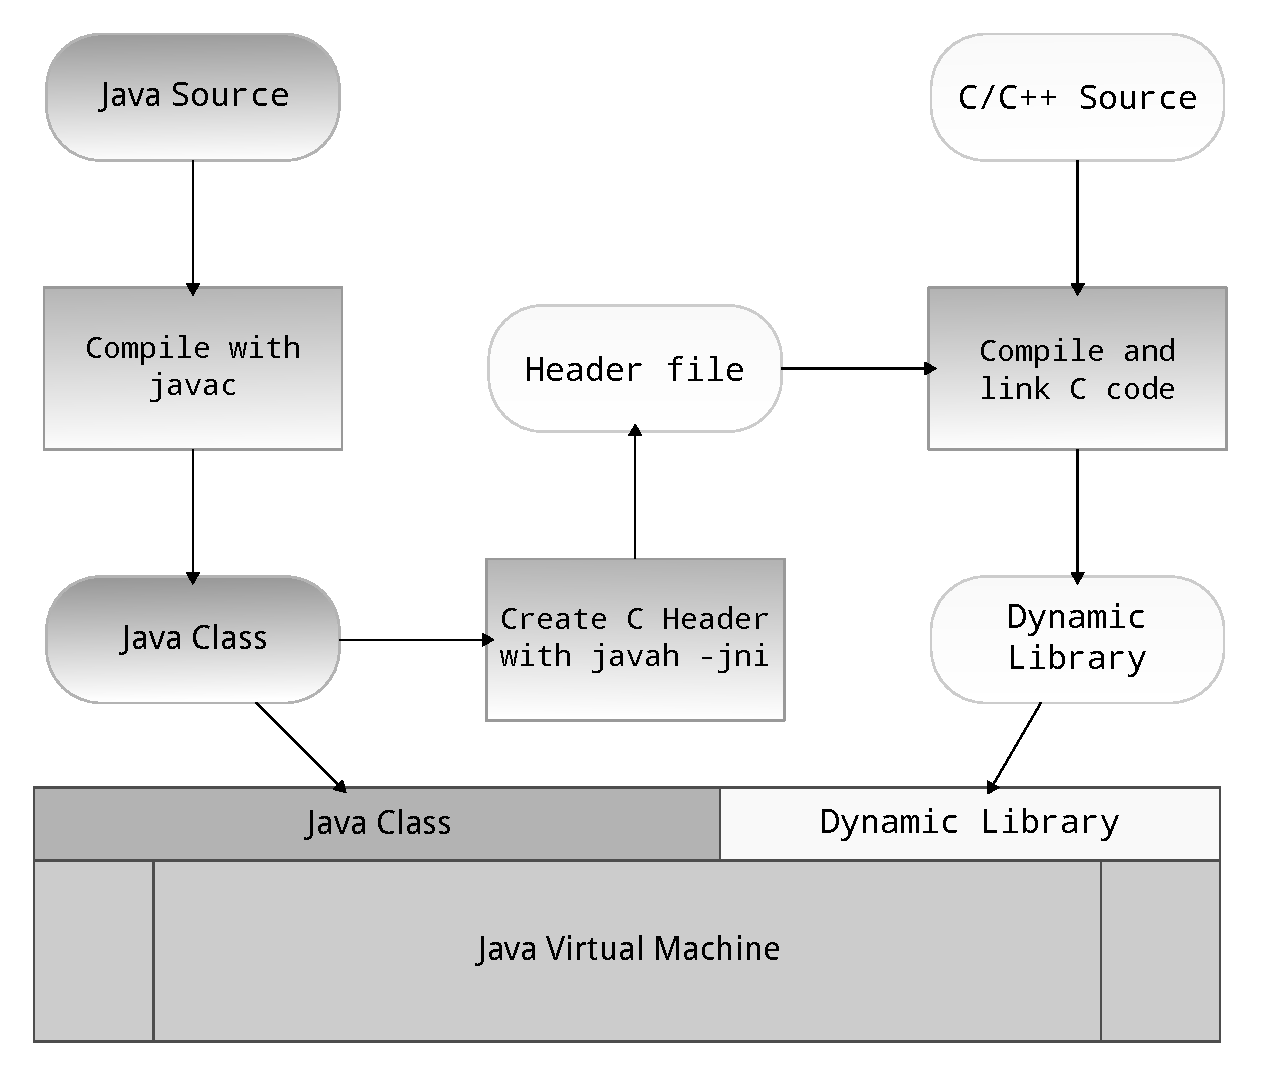
\includegraphics[width=8cm]{./figures/jni-flow.pdf}
 \caption{JNI flow}
 \label{fig:jni-flow}
\end{figurehere}

The focus of this work though points to explore JNI within the Android context,
therefore our starting point will be the Android NDK, which basically consists
of a ready-to-use tool-set (available on \url{http://developer.android.com/tools/sdk/ndk/index.html#Downloads}). The use
of the NDK condenses the steps above in just one main step, which will do almost
everything at once, through the \keyword{ndk-build} command.

%%%%%%%%%%%%%%%%%%%%%%%%%%%%%%%%%%%%%%%%%%%%%%%%%%%%%%%%%%%%%%%%%%%%%%%%%%%%%%%%

\section{Getting started}
\label{sec:getting-started}
Basically, to develop an "App" using the NDK, we need:
\begin{itemize}
\item Android SDK (\url{http://developer.android.com/sdk/index.html})
\item Android NDK (\url{http://developer.android.com/tools/sdk/ndk/index.html})
\item A source editor. Using Eclipse IDE for Java Developers automatises somehow
the building process. (\url{http://www.eclipse.org/downloads/})
\end{itemize}
From within the \textit{"SDK/tools"} directory, you can execute the \keyword{android} command, to launch the Android SDK Manager: from here, you can download Android API and Extras.\\
The Eclipse version you've downloaded will be a plain version, not yet customised to deal with specific Android needs and options: you then need to set up Android Tools for Eclipse by clicking \textit{"Help -> Install new software"} and putting the url \url{https://dl-ssl.google.com/android/eclipse/}.\\
Once the environment is set up, we are ready to start developing our fist, small, application, which will interact with a native c-written library. Instead of editing the java source code, and the native code separately, and then compiling them as shown in \reff{fig:jni-flow}, Eclipse will just (automatically) build the Java part, while we'll manually generate the native shared library (we'll see how to automatise this procedure at the end of this article).\\
The entirety of the files we'll work on (mainly, and at least two) is organised as shown below:

\dirtree{%
.1 .
.1 Tutorial1/.
.2 AndroidManifest.xml.
.2 jni/.
.3 Android.mk.
.3 tutorial1.c.
.2 res/.
.3 layout/.
.4 main.xml.
.3 values/.
.4 strings.xml.
.2 src/.
.3 com/.
.4 android/.
.5 tutorial1/.
.6 Tutorial1Activity.java.
}
Let's briefly analyse this structure, taking as example the \textbf{Tutorial1} at \refs{sec:tutorial1}.
\paragraph{Manifest}
\keyword{AndroidManifest.xml} is the file where the applications are described: here they declare the presence of content providers, services, required permissions and other elements.\\
In this simple case, it contains the basic nodes, which are:
\begin{itemize}
\item \keyword{manifest}: here, under the \keyword{package}, the Java package is specified. We use \keyword{com.android.tutorial1}
\item \keyword{uses-sdk}: here it's specified the minimum sdk version (we use API 16, which correspond to Android Jelly Bean)
\item \keyword{application}: general information about the application, a human-readable application label, icons.
\item \keyword{activity}: here we have the \keyword{android:name} full name of the activity (the java file), a \keyword{android:label} which is the name that will appear at the top of our running Activity, and the \keyword{<intent-filter>} node, which tells Android when this Activity should be run. Since our Tutorial1Activity will also be the one to be run after launch, we can declare this in the \keyword{<action>} node. When an App is called, Android looks for an activity that declares itself ready to resolve the \keyword{MAIN} action. In the second node, under the \keyword{<intent-filter>} node, we declare another attribute, which is \keyword{<category>}, where we specify that the category of our activity is \keyword{LAUNCHER}: this will allow the App to be launched from the Android desktop.
\end{itemize}
For the sake of clarity, the whole \keyword{AndroidManifest.xml} content is presented at \refl{lst:manifest-tut1}.

\begin{lstlisting}[language=XML,
				   columns=fullflexible,
				   showstringspaces=false,
				   commentstyle=\color{gray}\upshape,
				   caption=AndroidManifest.xml for Tutorial1,
				   label=lst:manifest-tut1]
<manifest
xmlns:android="http://schemas.android.com/apk/res/android"
       package="com.android.tutorial1"
       android:versionCode="1"
       android:versionName="1.0">
    <uses-sdk android:minSdkVersion="16" />
    <application android:label="Tutorial1"
                 android:debuggable="true">
        <activity android:name=".Tutorial1Activity"
        	   android:label="Tutorial1">
            <intent-filter>
                <action
                android:name="android.intent.action.MAIN"/>
                <category
                android:name="android.intent.category.LAUNCHER"/>
            </intent-filter>
        </activity>
    </application>
</manifest> 
\end{lstlisting}
\paragraph{Resources}
The \keyword{res} directory, contains, at least, the following subdirectories:
\begin{itemize}
\item \keyword{layout/}: This folder contains Android user interface XML files.\\
Without going into detail too much, here we can find each visible element that composes what we see on the screen: strings, buttons, tables, text fields, menus. An example of a button declaration can be seen below
\begin{lstlisting}[language=XML,
				   columns=fullflexible,
				   showstringspaces=false,
				   commentstyle=\color{gray}\upshape]
<Button android:layout_width="fill_parent"
	 android:layout_height="wrap_content"
	 android:id="@+id/button0"
	 android:text="@string/button0"
	 android:onClick="button0"/>
\end{lstlisting}
The \keyword{@+id/button0} and the \keyword{@string/button0} are references to other resources: the former will be used by the Java code to identify this specific button element, the latter identifies the value of the variable \keyword{button0} declared into the \keyword{strings.xml} file (see below)
\item \keyword{values/}: This folder contains values that the application will read during its execution, or static data an application will use for such purposes as internationalization of UI strings. In the \keyword{string.xml} file, we can declare the values corresponding to the \keyword{@string} definition, as shown below, for the \keyword{@string/button0} declared above:
\begin{lstlisting}[language=XML,
				   columns=fullflexible,
				   showstringspaces=false,
				   commentstyle=\color{gray}\upshape]
<string name="button0">Call to native</string>
\end{lstlisting}
\end{itemize}
These xml files will then be automatically built into an \keyword{R} object, visible to the activity, which will access to it and get views, and set values on its attributes.\\
When editing native JNI code in an Android project using the Android NDK you may
configure \textbf{Eclipse} to automatically rebuild your project when editing native code,
just as it does for java. Open your project \texttt{Properties}, then click \texttt{Builder} on the left hand side, and \texttt{New} on the right hand side. From the following dialog, choose \texttt{Program} and \texttt{OK}.\\
In the \texttt{Main} tab, we fill the fields as follows:
\begin{itemize}
\item Name: \texttt{NDK Builder}
\item \texttt{/opt/android-ndk/ndk-build} (or wherever your ndk-build binary is).
\item Working Directory:\\
\texttt{ \$ \{ workspace\_loc:/projectName \} } (Press the Browse Workspace... button to select it graphically)
\end{itemize}
Then we can switch to the second tab (\reff{fig:ndk-build-2}), \texttt{Refresh}: enable the option \texttt{"Refresh resources upon completion"} and click the button \texttt{Specify Resources...}: choose the \texttt{libs} directory within the workspace tree; be sure to check this folder only.

\begin{figurehere}
 \centering
 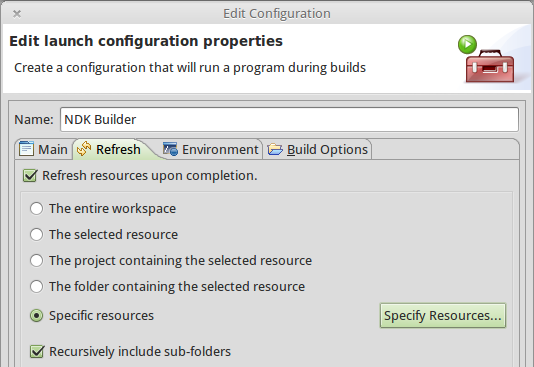
\includegraphics[width=7cm]{./figures/ndk-build-2.png}
 \caption{Refresh properties - Eclipse builder}
 \label{fig:ndk-build-2}
\end{figurehere}

The last tab, named \texttt{Build Options} is shown in \reff{fig:ndk-build-3}: as done for the \texttt{Refresh} tab, check the last option, and choose \texttt{Specify Resources...}. Choose the \texttt{jni} directory within your workspace tree; be sure to check this folder only.

\begin{figurehere}
 \centering
 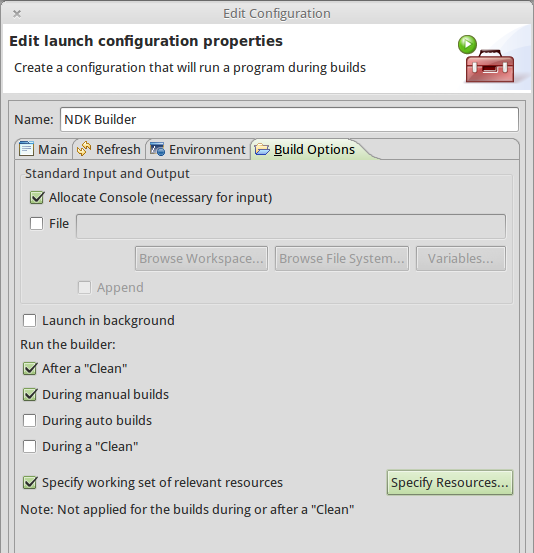
\includegraphics[width=7cm]{./figures/ndk-build-3.png}
 \caption{Build properties - Eclipse builder}
 \label{fig:ndk-build-3}
\end{figurehere}

This being done, the result of a project build (\texttt{ctrl+B}) is shown in \reff{fig:ndk-build-4}.

\begin{figurehere}
 \centering
 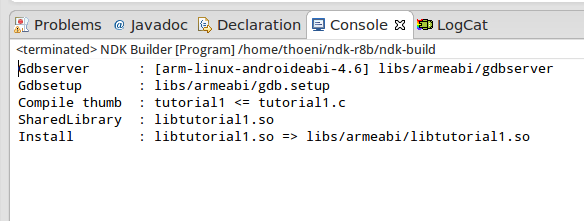
\includegraphics[width=7cm]{./figures/ndk-build-4.png}
 \caption{Native building result, into Eclipse console}
 \label{fig:ndk-build-4}
\end{figurehere}

%%%%%%%%%%%%%%%%%%%%%%%%%%%%%%%%%%%%%%%%%%%%%%%%%%%%%%%%%%%%%%%%%%%%%%%%%%%%%%%%

\section{Tutorial1}
\label{sec:tutorial1}
The complete code from this tutorial can be found at \url{https://github.com/thoeni/ndk-tutorials/tree/master/tutorial1}.\\
Eventually, after this brief introduction, we can get to the most interesting part of the tutorial: the Java activity, and the native code, which are respectively placed into the \keyword{src} and the \keyword{jni} directories.\\
The activity isn't any different from a regular Android activity except for two things: methods that correspond to native functions are declared as \keyword{native}, and a shared library is statically loaded by the \keyword{System.loadLibrary()} method.\\
Basically, this tutorial, illustrates how to call a native function from within the Java activity, and how to call the native function which, in turn, calls back the Java activity: the methods that perform these operations are, respectively \keyword{foo1(String)} and \keyword{foo2}, declared within the \keyword{Tutorial1Activity}, as shown in \refl{lst:tut1-java1}, line 1 and line 2.

\begin{lstlisting}[language=Java,
				   columns=fullflexible,
				   showstringspaces=false,
				   xleftmargin=15pt,
				   frame = l,
				   numbers=left,
				   commentstyle=\color{gray}\upshape,
				   caption=Part of Tutorial1Activity.java,
				   label=lst:tut1-java1]
public native String foo1(String message);
public native void foo2();
  
public void foo3Callback() {
   String message = "foo3Callback called back by foo2";
   output.setText(message);
}
  
static {
   System.loadLibrary("tutorial1");
}
\end{lstlisting}
In the same piece of code, we can see - line 4 - a regular \keyword{public void} method, named \keyword{foo3Callback()} which will be called by the native code, and - line 9 - the static declaration to load the shared library that will be generated by the \keyword{ndk-build} command.\\
For this first tutorial, we analyse entirely the native code. These are the basics of JNI, and later on, we won't need to specify everything this much: the C code can be seen at \refl{lst:tut1-c1}

\begin{lstlisting}[language=C,
				   columns=fullflexible,
				   showstringspaces=false,
				   xleftmargin=15pt,
				   frame = l,
				   numbers=left,
				   commentstyle=\color{gray}\upshape,
				   caption=tutorial1.c,
				   label=lst:tut1-c1]
#include <jni.h>
#include <android/log.h>

#include <stdio.h>
#include <stdlib.h>
#include <string.h>

#define  LOG_TAG    "tutorial1"
#define  LOGI(...)  __android_log_print(ANDROID_LOG_INFO,
				LOG_TAG,__VA_ARGS__)
#define  LOGE(...)  __android_log_print(ANDROID_LOG_ERROR,
				LOG_TAG,__VA_ARGS__)

jstring Java_com_android_tutorial1_Tutorial1Activity_foo1(
	JNIEnv* env, jobject thiz, jstring message) {
   //To print out a char* we have to convert
   //the jstring to char*
   const char *nativeString = (*env)->GetStringUTFChars(env,
				message, 0);
   LOGI("foo1 called! Input parameter: %s", nativeString);
   //Then we have to release the memory allocated for
   //the string
   (*env)->ReleaseStringUTFChars(env, message, nativeString);
   return (*env)->NewStringUTF(env, "JNI call J2C performed!");
}

void Java_com_android_tutorial1_Tutorial1Activity_foo2(
	JNIEnv* env, jobject thiz) {
   LOGI("foo2 called!");
   //Get class from the calling object
   jclass clazz = (*env)->GetObjectClass(env, thiz);
   if (!clazz) {
      LOGE("callback_handler: failed to get object Class");
      goto failure;
   }
   //Get the methodID from the class which the calling
   //object belongs
   jmethodID method = (*env)->GetMethodID(env, clazz,
   			"foo3Callback", "()V");
   if (!method) {
      LOGE("callback_handler: failed to get method ID");
      goto failure;
   }
   //Call the method on the calling object, defined by the
   //methodID
   (*env)->CallVoidMethod(env, thiz, method);

   failure: return;
}
\end{lstlisting}
The first thing that we can see is the \keyword{\#include <jni.h>} at line 1: this is the header file - included with the JDK - that maps Java types to their native counterparts (\reft{table:types-correspondence}).\\
There are two functions (line 14 and line 27): their names have a specific format which maps the full name of the "caller" Java class - where the \textit{underline} character replaces the typical Java \textit{dot notation} - and, at the end, there's the name of the function, which corresponds to the \keyword{native} method declared into our class.\\
Let's take \keyword{foo1} as example: the method declaration in \refl{lst:tut1-java1}\textbf{:1} is natively implemented in \refl{lst:tut1-c1}\textbf{:14}. As it's done for the name, the input parameters and the return type have to match as well, therefore we have that the java \keyword{String} type is mapped to a native \keyword{jstring} type (thanks to the jni.h library that we included some lines above); the same goes for the input (\keyword{String/jstring} again), with a peculiarity: native functions mapped to Java methods through JNI paradigm always have two more parameters, a \keyword{JNIEnv*} which is a pointer to the current Java environment, and a \keyword{jobject} which is a reference to the caller object. Given this, depending on the variety of input(s) and of the output type, we're able to properly create the correct JNI function declaration: from now on, with some attentions, native code can freely run.\\
In this tutorial I decided to pass a \keyword{String} as input to have the opportunity to show how the developer should proceed when she needs to handle variable types that are not primary ones. In this case, we have to explicitly convert the string from \keyword{jstring} to a \textit{"native-friendly"} \keyword{char*}: if you don't, the error is sometimes not as verbose as you would expect it to be, and it's quite hard to debug this situation, therefore pay attention to the Java/native types mismatch. As the reader can easily understand, we declare a native string, which will save the result of the right-hand side function (\refl{lst:tut1-c1}\textbf{:18}) \keyword{GetStringUTFChars} which obtains string characters represented in the Unicode format. The third parameter indicates whether we want a copy, or the pointer to the actual java string: in the latter case, the developer must pay attention not to modify the contents of the returned string. This parameter is typically set to NULL, and the JVM will autonomously determine the choice to pick.\\
We can finally log our parameter as \textit{information}. When the native code finishes using the UTF-8 string obtained through GetStringUTFChars, it calls ReleaseStringUTFChars, thus the memory taken by the UTF-8 string can be freed.\\
To satisfy the return type declared for this \keyword{foo1}, we return a new string. The procedure shown at \refl{lst:tut1-c1}\textbf{:24} is specific for generating a jstring object: we'll see further in this article that from the native code we are able to find java classes, instantiate them as jobjects, and call methods on them.\\
\keyword{foo2} function represents a very simple example of a JNI callback: typically, whenever we need to callback a Java method implemented into the class that made the call, we go through three main steps:
\begin{itemize}
\item get the class (\keyword{jclass}), starting from the object (\keyword{jobject}) which made the call, through the \keyword{GetObjectClass} \refl{lst:tut1-c1}\textbf{:31}
\item get the method identifier, through the \keyword{GetMethodID}, which performs a lookup for the method in the given class. The lookup is based on
the name and type descriptor of the method. If the method does not exist, \keyword{GetMethodID} returns \keyword{NULL} \refl{lst:tut1-c1}\textbf{:38}
\item call the method, on the caller object, passing the \keyword{methodID} \refl{lst:tut1-c1}\textbf{:46}
\end{itemize}
The code in \refl{lst:tut1-c1}\textbf{:27-49} is easy to read, despite for a detail that we are going to analyse: at line 38, the \keyword{GetMethodID} function, takes as input 4 parameters:
\begin{itemize}
\item \keyword{JNIEnv*}, the pointer to the Java environment
\item \keyword{jobject}, the caller object, that we passed to the native function as input parameter
\item \keyword{const char*}, the string which identifies the name of the method to call back
\item \keyword{const char*}, the "signature" of the method, called the method descriptor: despite it could seem bizarre, it's very easy to understand. The first part, between the round brackets, represents the input parameters, and their types; the last identifier, after the closed round bracket, represents the return type. In our case, \keyword{()V} means \keyword{void foo3Callback()}. If our function was, let's say, \keyword{float foo3Callback(int i)} we would write, as its descriptor: \keyword{(I)F}. And, again, with \keyword{float foo3Callback(int i, float f, int j)} we would write \keyword{(IFI)F}. A guide table is given at \reft{table:types-correspondence}. We will see how to declare complex descriptors, with strings, objects and arrays further.
\end{itemize}
\vspace{1em}
\begin{tablehere}
	\centering	
	\begin{tabular}{c l p{2cm}}
		\hline
		Signature & Java Type & Native Type \\
		\hline
		\texttt{Z} & \texttt{boolean} & \texttt{jboolean} \\
		\texttt{B} & \texttt{byte} & \texttt{jbyte} \\
		\texttt{C} & \texttt{char} & \texttt{jchar} \\
		\texttt{S} & \texttt{short} & \texttt{jshort} \\
		\texttt{I} & \texttt{int} & \texttt{jint} \\
		\texttt{L} & \texttt{long} & \texttt{jlong} \\
		\texttt{F} & \texttt{float} & \texttt{jfloat} \\
		\texttt{D} & \texttt{double} & \texttt{jdouble} \\
		\texttt{-} & \texttt{void} & \texttt{void} \\
		\hline
	\end{tabular}
	\caption{Types correspondence Java/JNI and signatures}
	\label{table:types-correspondence}
\end{tablehere}
\vspace{1em}
Signature for object and arrays are:\\
\vspace{1em}
\begin{tablehere}
	\centering
	\begin{tabular}{l l}
		\hline
		Signature & Java Type\\
		\hline
		\texttt{Lcom/qualified/class;} & \texttt{com-qualified-class}\\
		\texttt{[type} & \texttt{type[]}\\
		\hline
	\end{tabular}
\end{tablehere}

We still miss the last step, which allows the Java class to load the shared native library: the native code needs to be compiled by the \keyword{ndk-build} command. Before doing this, we have to create the \keyword{Android.mk} into the \keyword{jni} directory. The content of this file, for this tutorial, is shown at \refl{lst:tut1-c2}: after defining the name of the module that will be compiled, its source file, and local libs that we want to use, through the \keyword{include \$(BUILD\_SHARED\_LIBRARY)} instruction, we tell the compiler to create the shared object. Doing so, this library will be available to be loaded by Java classes. The use of \keyword{ndk-build} command is highly suggested, since it will generate all the files and folders that our environment needs.

\begin{lstlisting}[language=make,
				   columns=fullflexible,
				   showstringspaces=false,
				   xleftmargin=15pt,
				   frame = l,
				   numbers=left,
				   commentstyle=\color{gray}\upshape,
				   caption=Android.mk for tutorial1.c,
				   label=lst:tut1-c2]
LOCAL_PATH:= $(call my-dir)

include $(CLEAR_VARS)

LOCAL_MODULE    := tutorial1
LOCAL_CFLAGS    := -Werror
LOCAL_SRC_FILES := tutorial1.c
LOCAL_LDLIBS := -L$(SYSROOT)/usr/lib -llog

include $(BUILD_SHARED_LIBRARY)
\end{lstlisting}

An example of the activity performing a callback can be found at \reff{fig:tut1-scr1}: the output visible at the top of the screen comes from the Java method at \refl{lst:tut1-java1}\textbf{:5}\\

\begin{figurehere}
 \centering
 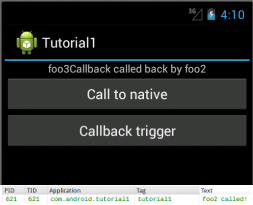
\includegraphics[width=6cm]{./figures/tut1-scr1.png}
 \caption{Tutorial1 performing a callback}
 \label{fig:tut1-scr1}
\end{figurehere}

So far we introduced the main components needed to develop within the Android NDK, and we saw a simple example where an activity calls - and is called back by - a native function.\\
In the next section, we'll add some features to this first example.

%%%%%%%%%%%%%%%%%%%%%%%%%%%%%%%%%%%%%%%%%%%%%%%%%%%%%%%%%%%%%%%%%%%%%%%%%%%%%%%%

\section{Tutorial2}
\label{sec:tutorial2}
The complete code from this tutorial can be found at \url{https://github.com/thoeni/ndk-tutorials/tree/master/tutorial2}.\\
Often we deal with threads, and we want to implement asynchronous calls from native to Java environment. Asynchronous calls are easy to do when the direction is Java to native, while the other way around - implemented through the callback mechanism - isn't that easy to figure out.\\
This example will consist of basic activity (almost identical to the one we used for \textit{Tutorial1}), that will be able to "run" and "stop" a routine. This routine will consist of a loop of four different callbacks, that will run into a thread: the loop exit condition is based on a flag that will be set and unset by the activity.\\
In addition to the basic blocks we saw for \textit{Tutorial1} at \refl{lst:tut1-java1}, we can find at \refl{lst:tut2-java1} the lines relevant to understand how \textit{Tutorial2} performs.
\begin{lstlisting}[language=Java,
				   columns=fullflexible,
				   showstringspaces=false,
				   xleftmargin=15pt,
				   frame = l,
				   numbers=left,
				   commentstyle=\color{gray}\upshape,
				   caption=Part of Tutorial2Activity.java source code,
				   label=lst:tut2-java1]
int int0;
float float0;
String string0;

public void onCreate(Bundle savedInstanceState) {
   // [...]
   init();
   handler = new Handler();
}

// [...]

public void callback1() {
   System.out.println("callback1 called");
   handler.post(callback1Thread);
}

Runnable callback1Thread = new Runnable() {
   @Override
   public void run() {
      output.setText("callback 1, no params");
   }
};

public int callback2(int param0, float param1,
                        String param2) {
   System.out.println("callback2 called, params are: "
      + param0 + " " + param1 + " " + param2);
   int0 = param0;
   float0 = param1;
   string0 = param2;
   handler.post(callback2Thread);
   return 0;
}

Runnable callback2Thread = new Runnable() {
   @Override
   public void run() {
      output.setText("callback 2, params are: "
         + int0 + ", " + float0 + ", " + string0);
   }
};

public void callback3(String param0) {
   System.out.println("callback 3, param is: "
      + param0);
   string0 = param0;
   handler.post(callback3Thread);
}

Runnable callback3Thread = new Runnable() {
   @Override
   public void run() {
      output.setText("callback 3, param is: " + string0);
   }
};

public float callback4(float param0) {
   System.out.println("callback 4, param is: " + param0);
   float0 = param0;
   handler.post(callback4Thread);
   return param0;
}

Runnable callback4Thread = new Runnable() {
   @Override
   public void run() {
      output.setText("callback 4, param is: " + float0);
   }
};

// [...]

public native void init();
public native void foo1();
public native void foo2();

static {
   System.loadLibrary("tutorial2");
}
\end{lstlisting}
At \refl{lst:tut2-java1}\textbf{:1-3} we declare three global variables where some callback values will be stored, and that will be accessed during some of the callbacks methods execution.\\
Within the \keyword{onCreate} method we call the first out of three native methods, named \keyword{init()}: the corresponding native function initialises some parameters and retrieves the various \keyword{methodIDs}.\\
Then callback methods declarations follow, at \refl{lst:tut2-java1}\textbf{:13-70}: for each callback method, there's a corresponding \keyword{Runnable} object which represents a command that can be executed, and is often used to run code in a different thread. This class declares an \keyword{abstract void} method, which therefore is mandatory to implement, and is the \keyword{run()} method: within this method we can put the active part of the code that must be executed and, typically, we use this to change the output view and display some values on the screen.\\
Below (\refl{lst:tut2-java1}\textbf{:74-76}) there are the declarations of three \keyword{native} functions.\\
Compared to the example we considered for the \textit{Tutorial1}, this native code is slightly more complex, and uses a thread and some JNI specific types we haven't had the chance to introduce before. To start, here we use the \keyword{JNI\_OnLoad} function (\refl{lst:tut2-c1}), which performs initialization operations for a given native library and returns the JNI version required by the native library. The virtual machine implementation calls \keyword{JNI\_OnLoad} when the native library is loaded, therefore we can use it to save a reference to the current Virtual Machine which - unlike the case of the \keyword{JNIEnv*} that is local to each call - lives along the whole life of the application.
\begin{lstlisting}[language=C,
				   columns=fullflexible,
				   showstringspaces=false,
				   xleftmargin=15pt,
				   frame = l,
				   numbers=left,
				   commentstyle=\color{gray}\upshape,
				   caption=Part of tutorial2.c - JNI\_OnLoad,
				   label=lst:tut2-c1]
static JavaVM *gJavaVM;				   
				   
jint JNI_OnLoad(JavaVM* vm, void* reserved)
{
  JNIEnv *env;
  gJavaVM = vm;
  LOGI("JNI_OnLoad called");
  if ( (*vm)->GetEnv(vm, (void**) &env, JNI_VERSION_1_4)
  		!= JNI_OK) {
     LOGE("Failed to get the environment using GetEnv()");
     return -1;
  }
  return JNI_VERSION_1_4;
}
\end{lstlisting}
The \keyword{init()} function saves global references to the caller object and, hence, to the caller class the objects belongs to. Besides it saves the references to the \keyword{methodIDs} statically declared into the \keyword{callback\_t} structure (specifically defined for this example).\\
In \refl{lst:tut2-c2} an extract of the structure declaration (\textbf{lines:1-15}), the global variables to save the global references to (\textbf{lines:17-18}), the same \keyword{GetMethodID} implementation we already saw (\textbf{line:35}) and the \keyword{NewGlobalRef()} function (\textbf{lines:26-28}), which creates a new global reference to the object referred to by the second argument. Global references must be explicitly disposed of by calling \keyword{DeleteGlobalRef}.\\
Since \keyword{init()} native method is called within the \keyword{onCreate}, this whole procedure will be executed the first time we run the activity, and when we launch it again after having destroyed it.\\
Now we can see what happens when the user calls \keyword{foo1}, and starts the testing routine.
\begin{lstlisting}[language=C,
				   columns=fullflexible,
				   showstringspaces=false,
				   xleftmargin=15pt,
				   frame = l,
				   numbers=left,
				   commentstyle=\color{gray}\upshape,
				   caption=Part of tutorial2.c - init(),
				   label=lst:tut2-c2]
callback_t cb[] = {
   // cb[0]
   {
     "callback1",
     "()V",
     JNI_WRAPPER_rVOID,
   },
   // cb[1]
   {
     "callback2",
     "(IFLjava/lang/String;)I",
     JNI_WRAPPER_rINT_p,
   },
   //[...]
};

static jobject gObject;
static jclass gClass;

void
Java_com_android_tutorial2_Tutorial2Activity_init(
				JNIEnv* env, jobject thiz)
{
   LOGI("init native function called");   
   //[...]   
   gObject = (jobject)(*env)->NewGlobalRef(env, thiz);
   jclass clazz = (*env)->GetObjectClass(env, thiz);
   gClass = (jclass)(*env)->NewGlobalRef(env, clazz);   
   //[...]   
   int i = sizeof cb / sizeof cb[0];
   //[...]   
   while(i--) {
   	LOGI("Method %d is %s with signature %s", i,
   			cb[i].cbName, cb[i].cbSignature);
   	cb[i].cbMethod = (*env)->GetMethodID(env, clazz,
   			cb[i].cbName, cb[i].cbSignature);
   }
}
\end{lstlisting}
\keyword{foo1} has no parameters, and its return value is void: its main code consists of a call to the function \keyword{daemonStart()}, therefore it's useless to show its code, though can be easily found on-line at the repository address. \keyword{daemonStart()}, in turn, creates a pthread and exits, and this is traditional C code, so far.\\
The function that is launched as thread is called \keyword{randomCaller()}, and uses the \keyword{gJavaVM} variable to retrieve the current \keyword{JNIEnv} and send it as input parameter to another function, which is a wrapper that, depending on the input parameters, chooses which method has to be called. A sequence diagram to clarify its working is shown in \reff{fig:tut12-seq}.
\begin{figure*}[t]
 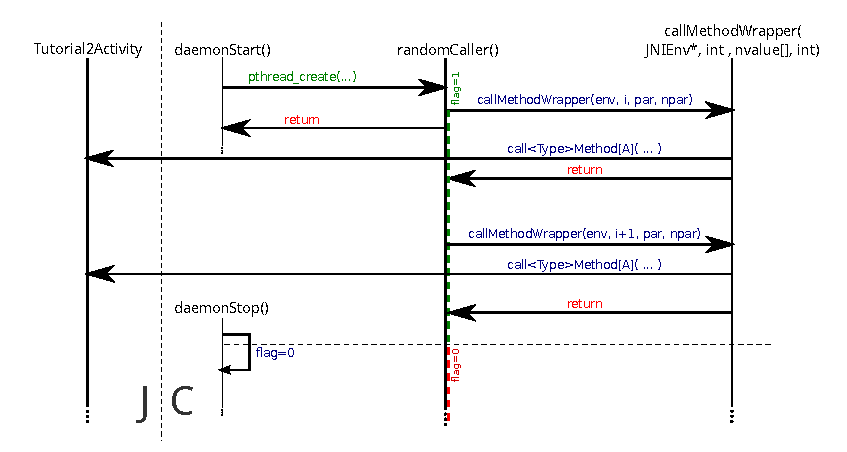
\includegraphics[width=17cm]{./figures/sequence.pdf}
 \caption{Tutorial2 sequence diagram}
 \label{fig:tut12-seq}
\end{figure*}
Unlike \textit{Tutorial1}, this example uses a thread, and there's a proper procedure to \textit{attach} the current thread to the JVM, as shown in \refl{lst:tut2-c3}.
\begin{lstlisting}[language=C,
				   columns=fullflexible,
				   showstringspaces=false,
				   xleftmargin=15pt,
				   frame = l,
				   numbers=left,
				   commentstyle=\color{gray}\upshape,
				   caption=Part of tutorial2.c - thread attachment in randomCaller(),
				   label=lst:tut2-c3]
void *randomCaller() {
   flag = 1;
   JNIEnv *env;
   int isAttached = 0;				   
   int status = (*gJavaVM)->GetEnv(gJavaVM, (void **) &env,
		JNI_VERSION_1_4);
   if(status < 0) {
      LOGE("callback_handler: failed to get JNI environment,
      		assuming native thread");
      status = (*gJavaVM)->AttachCurrentThread(gJavaVM, &env,
      							NULL);
      if(status < 0) {
         LOGE("callback_handler: failed to attach current
         	thread");
      }
   isAttached = 1;

   /*
   * callMethodWrapper(i++) 
   * sleep(2);   
   */
   
   if(isAttached)
      (*gJavaVM)->DetachCurrentThread(gJavaVM);
}
\end{lstlisting}
At \refl{lst:tut2-c3}\textbf{:5} is called the \keyword{GetEnv} function on the global reference of the JVM: this function sets \keyword{*env} to \keyword{NULL} if the current thread is not attached to the given virtual machine instance, and returns \keyword{JNI\_EDETACHED} which corresponds to \keyword{-2}; if the specified interface is not supported, it sets \keyword{*env} to \keyword{NULL}, and returns \keyword{JNI\_EVERSION} which corresponds to \keyword{-3}. Otherwise, sets \keyword{*env} to the appropriate interface, and returns \keyword{JNI\_OK}, which corresponds to \keyword{0}. Since we know we are running this code within a thread, the status value will be \keyword{-2}, and the thread attachment will be attempted (\refl{lst:tut2-c3}\textbf{:10}): the \keyword{AttachCurrentThread} function sets up the current native thread to run as part of a virtual machine instance. Once a thread is attached to the virtual machine instance, it can then make JNI function calls to perform such tasks as accessing objects and invoking methods. The \keyword{DetachCurrentThread} function (\refl{lst:tut2-c3}\textbf{:24}) informs a virtual machine instance that the current thread no longer needs to issue JNI function calls, allowing the virtual machine implementation to perform clean-ups and free resources.\\
How the \keyword{switch} condition works inside the \keyword{randomCaller} is easy to understand (\refl{lst:tut2-c3}\textbf{:18-21}), hence the full code isn't presented in this paper, nonetheless it's important to stress the peculiarity of a calling method, which is the \keyword{call<Type>MethodA()} \refl{lst:tut2-c5}\textbf{:24}: to test this cycle, the \keyword{randomCaller} defines some variables, and calls the wrapper passing four arguments to it. An example about this can be seen in \refl{lst:tut2-c4}: at \textbf{line:11} the developer sets as input parameters the env variable, the ordinal number of the chosen callback method (\refl{lst:tut2-c2}\textbf{:9-13}), the array of native params (which is a \keyword{struct} we defined) and the size of this array.
\begin{lstlisting}[language=C,
				   columns=fullflexible,
				   showstringspaces=false,
				   xleftmargin=15pt,
				   frame = l,
				   numbers=left,
				   commentstyle=\color{gray}\upshape,
				   caption=Part of tutorial2.c - method calls in randomCaller(),
				   label=lst:tut2-c4]
nvalue v1, v2, v3, npar[3];
v1.type = INT;
v1.i = 12;
v2.type = FLOAT;
v2.f = 2.3;
v3.type = STRING;
v3.s = "string";
npar[0] = v1;
npar[1] = v2;
npar[2] = v3;
callMethodWrapper(env, 1, npar, 3);
\end{lstlisting}
The \keyword{callMethodWrapper} function is partially shown in \refl{lst:tut2-c5}: the \keyword{for} at \textbf{line:7} maps all the native values to \keyword{jvalue[]}, which is a \keyword{struct} already defined for the JNI environment. It comes quite useful in this case because we can take advantage of the \keyword{call<Type>MethodA} function, where the \keyword{A} at the end of its name means that it takes as fourth parameter an \keyword{jvalue} array.

\begin{figure*}[t]
 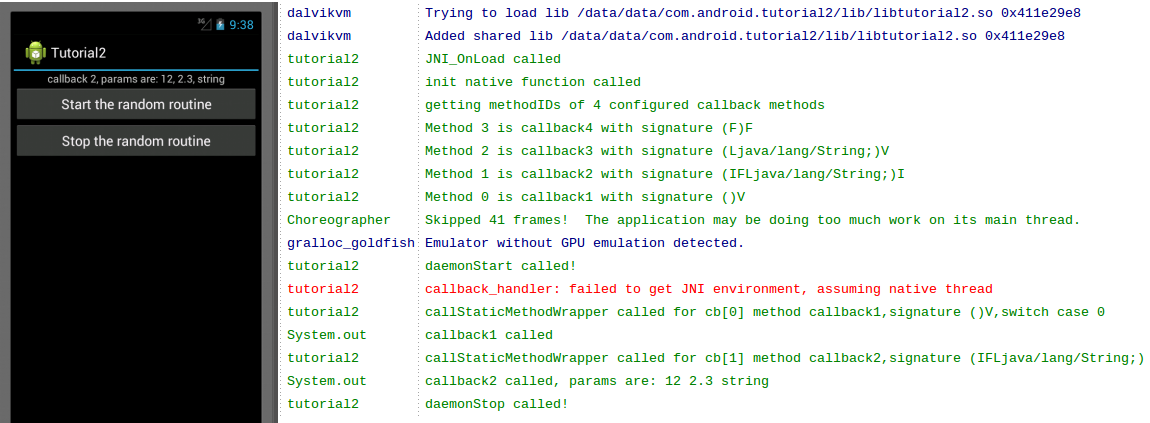
\includegraphics[width=17cm]{./figures/tut2-scr1.png}
 \caption{Tutorial2 running example}
 \label{fig:tut2-scr1}
\end{figure*}
\begin{lstlisting}[language=C,
				   columns=fullflexible,
				   showstringspaces=false,
				   xleftmargin=15pt,
				   frame = l,
				   numbers=left,
				   commentstyle=\color{gray}\upshape,
				   caption=Part of tutorial2.c - callingMethodWrapper,
				   label=lst:tut2-c5]
int callMethodWrapper(JNIEnv* env, int mid, nvalue npar[],
			int parSize) {
   jvalue jpar[parSize];
   //[ ... ]
   if (parSize > 0) {
   int i;
   for (i=0; i<parSize; i++) {
      switch (npar[i].type) {
         case INT:
            jpar[i].i = npar[i].i;
         break;
         case FLOAT:
            jpar[i].f = npar[i].f;
         break;
         case STRING:
            jpar[i].l = (*env)->NewStringUTF(env, npar[i].s);
         break;
      }
   }
}
switch (cb[mid].jniWrapper) {
   //[ ... ]
   case JNI_WRAPPER_rINT_p:
      (*env)->CallIntMethodA(env, gObject, cb[mid].cbMethod,
      				jpar);
   break;
   //[ ... ]
}
\end{lstlisting}
A screenshot of \textit{Tutorial2} activity and logcat during the execution can be found at \reff{fig:tut2-scr1}

%%%%%%%%%%%%%%%%%%%%%%%%%%%%%%%%%%%%%%%%%%%%%%%%%%%%%%%%%%%%%%%%%%%%%%%%%%%%%%%%

\section{Java object handling within native code}
It's possible that you would need to pass to the Java world a reference to an object that doesn't exist yet.\\
We'll analyse how it's possible to find a class, create an instance of this class, and call some methods on it.\\
Let's suppose we created a class, called Param, within the \keyword{tutorial2} package, which looks like the one in \refl{lst:tut2b-java1}
\begin{lstlisting}[language=Java,
				   columns=fullflexible,
				   showstringspaces=false,
				   xleftmargin=15pt,
				   frame = l,
				   numbers=left,
				   commentstyle=\color{gray}\upshape,
				   caption=Java class Param,
				   label=lst:tut2b-java1]
package com.android.tutorial2;

public class Param {
	private int[] iParams;
	private float[] fParams;
	private String[] sParams;

	public Param(int[] iP, float[] fP, String[] sP) {
		setiParams(iP);
		setfParams(fP);
		setsParams(sP);
	}

	public int[] getiParams() {
		return iParams;
	}
	public void setiParams(int[] iParams) {
		this.iParams = iParams;
	}
	public String[] getsParams() {
		return sParams;
	}
	public void setsParams(String[] sParams) {
		this.sParams = sParams;
	}

	public float[] getfParams() {
		return fParams;
	}
	public void setfParams(float[] fParams) {
		this.fParams = fParams;
	}
}
\end{lstlisting}
Suppose that we need to create a Param object, assign some values to its fields, and pass its reference to a Java method through the callback mechanism. Let's see the main steps to achieve this aim.\\
To begin, we need to get a reference to the \keyword{Param} class, and we do this as follow:
\begin{lstlisting}[language=C,
				   columns=fullflexible,
				   showstringspaces=false,
				   xleftmargin=15pt,
				   frame = l,
				   numbers=left,
				   commentstyle=\color{gray}\upshape]
//Find the "Param" Class
cls = (*env)->FindClass(env, "com/android/tutorial2/Param");
\end{lstlisting}
We can then create java arrays and, depending on the type of array we are going to create, we have to use a different constructor function, for instance, to create a \keyword{jint} array:
\begin{lstlisting}[language=C,
				   columns=fullflexible,
				   showstringspaces=false,
				   xleftmargin=15pt,
				   frame = l,
				   numbers=left,
				   commentstyle=\color{gray}\upshape]
int isize = 3;
jint iparams[isize] = {0, 1, 2};
//###Create a new Array of integers###
iarr = (*env)->NewIntArray(env, isize);
//Fill the array with the integer input parameter
(*env)->SetIntArrayRegion(env, iarr, 0, isize, iparams);
\end{lstlisting}
Now the object \keyword{iarr} is a Java array of integers.\\
The same thing can be done for floats, as follows:
\begin{lstlisting}[language=C,
				   columns=fullflexible,
				   showstringspaces=false,
				   xleftmargin=15pt,
				   frame = l,
				   numbers=left,
				   commentstyle=\color{gray}\upshape]
int fsize = 2;
jfloat fparams[fsize] = {1.2, 3.2};
//###Create a new Array of floats###
farr = (*env)->NewIntArray(env, fsize);
//Fill the array with the float input parameter
(*env)->SetFloatArrayRegion(env, farr, 0, fsize, fparams);
\end{lstlisting}
Now, for the \keyword{String} we don't have any ready-to-use function to create an array of \keyword{String} objects, therefore we can use the more general \keyword{NewObjectArray} function, as follows:
\begin{lstlisting}[language=C,
				   columns=fullflexible,
				   showstringspaces=false,
				   xleftmargin=15pt,
				   frame = l,
				   numbers=left,
				   commentstyle=\color{gray}\upshape]
int ssize = 2;
char* sparams[ssize] = {"ab","cd"};
sarr = (*env)->NewObjectArray(
		env, ssize, (*env)->FindClass(
				env, "java/lang/String"), NULL);
for (i=0; i<ssize; i++)
   (*env)->SetObjectArrayElement(
   		env, sarr, i, (*env)->NewStringUTF(
   				env, sparams[i]));
\end{lstlisting}
Now, we have three Java arrays correctly initialised: we can create an object of the \keyword{Param} class, and use its constructor (\refl{lst:tut2b-java1}\textbf{:8}) to initialise it with these newly generated arrays:
\begin{lstlisting}[language=C,
				   columns=fullflexible,
				   showstringspaces=false,
				   xleftmargin=15pt,
				   frame = l,
				   numbers=left,
				   commentstyle=\color{gray}\upshape]
jmethodID constructor;
//Find the constructor of the Param object, which takes as
//parameter an int array and a float array
constructor = (*env)->GetMethodID(env, cls, "<init>",
		"([I[F[Ljava/lang/String;)V");
//Create the Object with its constructor, and the arrays as
//parameters
obj = (*env)->NewObject(
		env, cls, constructor, iarr, farr, sarr);
//Call the callback method passing the object as input
//parameter
(*env)->CallStaticVoidMethod(
		env, gClass, cb[id].cbMethod, obj);
\end{lstlisting}
As we saw in \refs{sec:tutorial1}, the following signature \keyword{"([I[F[Ljava/lang/String;)V"} indicates a method - in this case \keyword{<init>} identifies the constructor method - which has a \keyword{void} return, and has input structured like:
\begin{itemize}
\item \keyword{[I} -> array of integers: int[]
\item \keyword{[F} -> array of floats: float[]
\item \keyword{[Ljava/lang/String;} -> array of objects \keyword{L} indicates object, of type \keyword{java/lang/String}: String[]
\end{itemize}
Therefore this signature means \keyword{void <init> (int[], float[], String[])}, which is exactly how the \keyword{Param} constructor is defined at \refl{lst:tut2b-java1}\textbf{:8}.

%%%%%%%%%%%%%%%%%%%%%%%%%%%%%%%%%%%%%%%%%%%%%%%%%%%%%%%%%%%%%%%%%%%%%%%%%%%%%%%%

\section{Tutorial3}

For this tutorial, we apply all we've seen so far, adding some concepts that can
let us taking advantage of the native code though some mechanisms which are
typical of Android: we'll introduce a Service, and two different messaging
systems, to enable a communication channel between the Activity and the Service.
\\Doing so, we'll decouple the \keyword{View} (the activity) and the \keyword{Controller} (the service): the
only interface to the Native environment will be the Service, and the Activity
will be used only as a "trigger" for Java calls to Native, and as a "display" of calls coming from the Service (and, to it, from the Native). A sample sequence diagram of this tutorial can be found at \reff{fig:tut3-seq}

\begin{figure*}[b]
 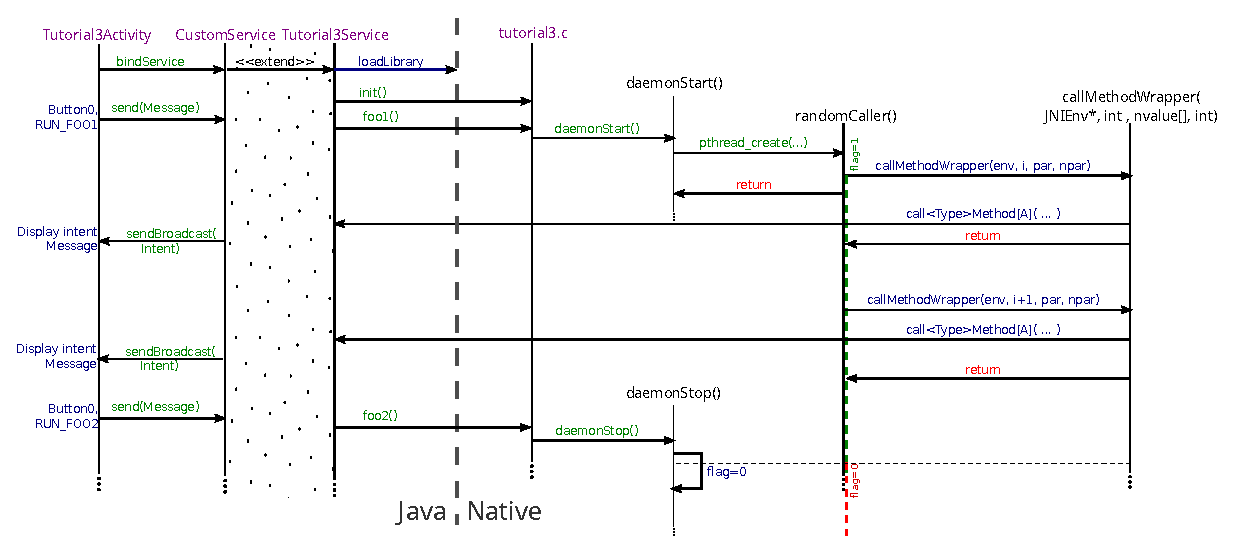
\includegraphics[width=17cm]{./figures/sequence_t3.pdf}
 \caption{Tutorial3 sequence diagram}
 \label{fig:tut3-seq}
\end{figure*}

%%%%%%%%%%%%%%%%%%%%%%%%%%%%%%%%%%%%%%%%%%%%%%%%%%%%%%%%%%%%%%%%%%%%%%%%%%%%%%%%

\section{Conclusions}

This report and all the source code are publicly available through the git
repository at \url{https://github.com/thoeni/ndk-tutorials} or at \url{https://bitbucket.org/atroina/ndk-tutorials}.

%%%%%%%%%%%%%%%%%%%%%%%%%%%%%%%%%%%%%%%%%%%%%%%%%%%%%%%%%%%%%%%%%%%%%%%%%%%%%%%%
% No cited references 
\nocite{liang1999jni}
\nocite{marakanajni}
\nocite{learningandroid}
\nocite{programmingandroid}

% We suggest the use of JabRef for editing your bibliography file (Report.bib)
\bibliographystyle{splncs}
\bibliography{Report}

\end{multicols}
\end{document}
